\documentclass[onecolumn]{gwclass}
\usepackage[utf8]{inputenc}
\newcommand{\definition}{\boxdefinition}  % this class names it \boxdefinition

\usepackage{tikz-cd}


\usepackage{graphicx}
\usepackage{wrapfig}
\graphicspath{{img/}}






\title{\vspace{2in}\Huge\textbf{Linear Algebra}}
\author{--- George Willingham ---}
\date{}

\begin{document}
	

\maketitle

\newpage
\tableofcontents


\newpage
\section{Vector Spaces}
\subsection{Introduction}

These notes are intended to be a practical guide to the subject of linear algebra. By ``practical", I mean that the end goal is to be able to use concepts from linear algebra in an applied setting (physics, optimization, signal processing, statistics, machine learning, etc.). However, that said, there will be several times in these notes where I cannot help but go a bit deeper to try and expose the real power and marvel of linear algebra. In such times, I will aim to show that, in its full abstraction, it is \emph{not} just the study of matrices as is often thought, but instead has a far more vast domain of applicability. It is in fact the study of \textbf{linearity} in all its guises.
 
 All of linear algebra takes place in \textbf{vector spaces}. Intuitively, a vector space is just like the real 3-dimensional space we live in --- we may call it $\mathbb{R}^3$. Every point in space corresponds to a \textbf{vector} which we write in bold notation $\*x \in\mathbb{R}^3$. With a choice of coordinates, every vector has \textbf{components} $x_1,x_2,x_3$. Trivially generalizing to $n$-dimensional space, we write a vector in $\mathbb{R}^n$ as
 $$ \*x=\begin{pmatrix}
 	x_1 \\
 	x_2 \\
 	\vdots \\
 	x_n
 \end{pmatrix}\in\mathbb{R}^n $$
 The $x_i$ are the coordinates, or components, of the vector and we conventionally write this as a \textbf{column vector} where the coordinates are stacked vertically\footnote{The role of \emph{row vectors} will be discussed later on.}. So this is what the elements of a vector space look like, but importantly, a vector space is not just the bare set $\mathbb{R}^n$ --- it has additional algebraic structure. Vectors can be multiplied by a scalar $a\*x$ which just scales all the coordinates and they can also be summed $\*x + \*y$ which acts entry-wise:
 $$ a\*x = \begin{pmatrix}
 	ax_1 \\
 	ax_2 \\
 	\vdots \\
 	ax_n
 \end{pmatrix}\qquad\qquad\qquad\qquad \*x + \*y = \begin{pmatrix}
 	x_1 + y_1 \\
 	x_2 + y_2 \\
 	\vdots \\
 	x_n + y_n
 \end{pmatrix} $$
\begin{wrapfigure}[13]{r}{0.3\textwidth}
	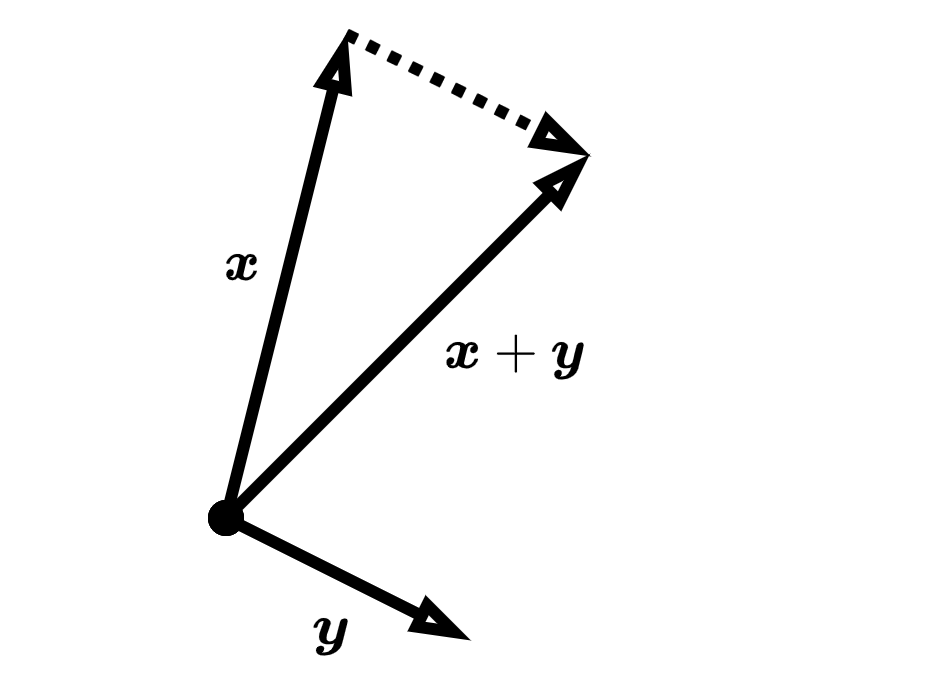
\includegraphics[scale=0.8]{vector_addition.drawio.png}
	\caption{Vector addition can be viewed as attaching arrows ``head to tail".}
\end{wrapfigure}
These are the fundamental operations for a vector space and all of linear algebra will be built on top of them. They satisfy many natural conditions such as associativity, commutativity, and distributivity\footnote{These properties are outlined in detail in the later section on the abstract definition of a vector space.}. 

In introductory physics courses, vectors are often described as quantities which have both \emph{size} and \emph{direction} and as such can be thought of as arrows. This is a valid way of thinking--- every point in space corresponds to an arrow pointing from the origin to that point. Scaling a vector $\*x$ by $a$ has the simple interpretation of stretching/shrinking the length of the arrow by a factor of $a$. Vector addition admits a similarly nice geometric interpretation. Treating vectors $\*x$ and $\*y$ as arrows from the origin, the sum $\*x+\*y$ is obtained by attaching $\*y$ to the end of $\*x$. This is illustrated to the right in Figure 1.


\newpage
\subsection{Span \& Linear Independence}


With the fundamental operations of scalar multiplication and vector addition, we can form \textbf{linear combinations} of vectors $\*x_1,\dots,\*x_n$ to get new vectors. A linear combination is of the form
$$  a_1\*x_1 + \dots + a_n\*x_n $$
for some scalar coefficients $a_1,\dots,a_n$. Naturally, combining vectors in this way always yields another vector in our space. If we consider all possible coefficients in this combination, we get the \textbf{span} of the set of vectors $\*x_1,\dots,\*x_n$. We have the following definition:
\definition{Span}{A set of vectors $\*x_1, \*x_2,\dots,\*x_k$ has \textbf{span} defined by all possible linear combinations of those vectors. That is,
$$ \t{span}\{ \*x_1,\dots,\*x_k \} \equiv \{ \t{all linear combinations } a_1\*x_1 + a_2\*x_2 + \dots + a_k\*x_k \} $$}
Consider as an example, the vectors $\*e_1=\tiny\begin{pmatrix}
	1\\0\\0
\end{pmatrix}$, $\*e_2=\tiny\begin{pmatrix}
0\\1\\0
\end{pmatrix}$, and $\*e_3=\tiny\begin{pmatrix}
0\\0\\1
\end{pmatrix}$ which all live in $\mathbb{R}^3$. We can clearly write any $\*x\in\mathbb{R}^3$ as a linear combination of these vectors:
$$ \begin{pmatrix}
	x_1\\x_2\\x_3
\end{pmatrix} = x_1\*e_1 + x_2\*e_2 + x_3\*e_3 $$
This means that $\t{span}\{\*e_1,\*e_2,\*e_3\}=\mathbb{R}^3$. But if instead, we only consider $\*e_1$ and $\*e_2$, it is not difficult to see that $\t{span}\{\*e_1,\*e_2\}$ is just the $xy$-plane. This is a 2-dimensional vector space that lives inside of $\mathbb{R}^3$. It is a \textbf{subspace} equivalent to $\mathbb{R}^2$. Importantly however, the span of $n$ vectors is \textbf{not} necessarily an $n$-dimensional vector space. To see this, consider the span of three vectors: $\*e_1, \*e_2$, and their linear combination $\*e_1+\*e_2$. A vector in $\t{span}\{\*e_1,\*e_2,\*e_1+\*e_2\}$ has the form
$$ a\*e_1 + b\*e_2 + c(\*e_1 + \*e_2) = (a+c)\*e_1  + (b+c)\*e_2 $$
for some coefficients $a,b,c$. Evidently then, it seems that every vector in this space is equivalently just a linear combination of $\*e_1$ and $\*e_2$ so we can write
$$ \t{span}\{\*e_1,\*e_2,\*e_1+\*e_2\} = \t{span}\{\*e_1,\*e_2\} $$
So the span of these three vectors is actually only a 2-dimensional space. The problem is that since $\*e_1+\*e_2$ is a linear combination of the other vectors, we could absorb its coefficients into the coefficients for $\*e_1$ and $\*e_2$. This example illustrates that for the span of $n$ vectors to be fully $n$-dimensional, we must not be able to write any of those vectors as a linear combination of the others. This is the important concept of \textbf{linear independence} and we define it now.
\definition{Linear Independence}{A set of vectors $\*x_1,\*x_2,\dots,\*x_n$ is \textbf{linearly dependent} if any one of them is a linear combination of the others, i.e. if there is an $\*x_k$ in the set such that
$$ \*x_k = a_1\*x_1 + \dots + a_{k-1}\*x_{k-1} + a_{k+1}\*x_{k+1} + \dots + a_n\*x_n $$ 
for some coefficients $a_1,\dots,a_n$. A set of vectors is \textbf{linearly independent} if they are not linearly dependent.}
Another way of viewing linear independence is to rearrange the above linear combination and consider coefficients which solve the equation
$$ a_1\*x_1 + \dots + a_n\*x_n = \*0 $$
The vectors $\*x_1,\dots,\*x_n$ are linearly independent if and only if the only solution to this is the trivial solution ($a_1=a_2=\dots=a_n=0$). Indeed, if a nontrivial solution exists, then we could simply rearrange to write one vector as a linear combination of the others. This definition of linear independence will be used later in these notes and will serve as a more operational definition.
\subsection{Basis}

With span and linear independence defined, we can move on to discuss the important concept of a basis. 
\definition{Basis}{A \textbf{basis} of a vector space $V$ is a set of linearly independent vectors $\*x_1,\dots,\*x_n\in V$ which span the full space. That is,
$$ \t{span}\{\*x_1,\dots,\*x_n\} = V $$}
With this terminology, we can say that $\*e_1, \*e_2$, and $\*e_3$ form a basis of $\mathbb{R}^3$. While this is the most obvious basis, there are others. In fact, there are infinitely many bases for any vector space but they all contain the same number of vectors. Another simple basis of $\mathbb{R}^3$ is $\*e_1,\*e_1+\*e_2$, and $\*e_3$. In this case, we have $\*x = (x_1-x_2)\*e_1 + x_2(\*e_1 + \*e_2) +x_3\*x_3$. Or more explicitly:
$$ \begin{pmatrix}
	x_1\\x_2\\x_3
\end{pmatrix} = (x_1-x_2)\begin{pmatrix}
1 \\0\\0
\end{pmatrix} + x_2\begin{pmatrix}
1\\1\\0
\end{pmatrix} + x_3\begin{pmatrix}
0\\0\\1
\end{pmatrix}$$
At this point, we must make an important conceptual leap. Consider that so far, when we write a vector as having components $x_1,x_2,x_3$, we have been implicitly using the \textbf{standard basis} $\*e_1,\*e_2,\*e_3$ to define those components. They are nothing other than the coefficients which allow us to write the linear combination $\*x=x_1\*e_1 + x_2\*e_2 + x_3\*e_3$. But there is nothing that makes this choice of basis special. We could just as well use the $\*e_1,\*e_1+\*e_2,\*e_3$ basis to define the components of the vector so that $\*x$ would look like 
$$ \*x = \begin{pmatrix}
	x_1-x_2\\x_2\\x_3
\end{pmatrix} $$
While this appears to be a different vector from the one with components $x_1,x_2,x_3$, it is the \textbf{same vector} --- we have simply chosen a different way to represent it! In this way, a choice of basis is really a choice of coordinate system. With an arbitrary vector $\*x$, we choose which set of basis vectors we will use to write $\*x$ as a linear combination. Then the coefficients in that combination define the components of $\*x$.  

The conceptual leap here is to realize that a vector is \textbf{not} defined by its components. They can change with a different choice of basis, but the underlying vector is a geometric object which is independent of how we choose to describe it. A vector is \emph{not} just a list of values, but it can be represented as a list of values once we choose a basis.

\newpage


\subsection{Abstract Definition of a Vector Space}

Thinking of vector spaces as a generalization of ordinary space is a perfect motivation for vector spaces, but all of this is just a concrete description of the more abstract algebraic definition. The proper definition of a vector space is given below:
\definition{Vector Space}{A vector space over a field\footnote{$\mathbb{K}$ is either $\mathbb{R}$ or $\mathbb{C}$ for our purposes} $\mathbb{K}$ is a set $V$ along with the operations of vector addition and scalar multiplication which satisfy the following axioms. For any $\*u,\*v,\*w \in V$ and any $a,b\in \mathbb{K}$:
	\begin{itemize}
		\setlength\itemsep{0.1em}
		\item Associativity of vector addition: $(\*u + \*v) + \*w = \*u + (\*v+\*w)$
		\item Commutativity of vector addition: $\*u+\*v=\*v+\*u$
		\item There exists an identity element (zero vector) $\*0$ such that $\*u+\*0=\*u$
		\item For every $\*u$, there exists an inverse $-\*u$ such that $\*u + (-\*u)=\*0$
		\item Scalar multiplication is compatible with field multiplication $a(b\*u)=(ab)\*u$
		\item There is a scalar identity $1\*u=\*u$
		\item Distributivity of scalar multiplication w.r.t vector addition $a(\*u+\*v)=a\*u +a\*v$
		\item Distributivity of scalar multiplication w.r.t field addition $(a+b)\*u=a\*u + b\*u$
\end{itemize}}
With this definition in hand, there are many spaces which at first glance are not obviously identified as vector spaces. For example, consider the set of all polynomials of degree 2: functions of the form $p(x)=ax^2 + bx + c$ for constant real coefficients $a,b,c$. It is easy to show that in fact all such polynomials form a vector space. Just consider that if $p_1$ and $p_2$ are degree 2 polynomials, then so is $p_1(x)+p_2(x)$ and so is any scaling of them. This particular space is equivalent to $\mathbb{R}^3$ since it can be identified as having coordinates $a,b,c$. This is just one example from the more general topic of \textbf{function spaces} --- the study of which is called functional analysis.\footnote{The reader interested in quantum mechanics or signal processing should absolutely familiarize themselves with functional analysis. It is a beautiful subject with deep ties to PDEs and harmonic analysis.} 

Note that a vector product $\*x\times\*y=\*z\in \mathbb{R}^n$ is \textbf{not} defined for a vector space on its own. In fact, when a vector space is endowed with a well-behaved vector product like this, it is known as \emph{an algebra} (a potentially confusing bit of terminology). The theory of algebras in this sense is rich and useful but will not be the topic of these notes save for a few notable exceptions.
\vfill
\section*{}

\newpage
\section{Linear Maps \& Matrices}
\subsection{Linearity}

With vector spaces defined, we need one more concept to dive into linear algebra: \textbf{linear maps}. We begin with the definition of linearity:
\definition{Linearity}{A map $f:U\to V$ is called \textbf{linear} if it has the following two properties
	\begin{itemize}
		\setlength\itemsep{0.1em}
		\item $f(a\*x) = af(\*x)$ 
		\item $f(\*x+\*y) = f(\*x)+f(\*y)$
	\end{itemize}
	for any scalar $a$ and any $\*x,\*y\in U$.}
Consider a few examples. A function $g:\mathbb{R}^n\to\mathbb{R}$ which takes a vector in $\mathbb{R}^n$ and returns a linear combination of its components as $ g(\*x) = a_1x_1 + \dots + a_nx_n $ is easily shown to be a linear map. However, if we add a constant to this, it becomes non-linear, i.e. the map $h(\*x)=g(\*x) + a_0$ is nonlinear. Any function which involves higher powers (e.g. $x^2, x^3,$ etc.) is also nonlinear. Other examples of linear maps include differentiation and integration of functions. That is, the map which takes a function $u$ to its derivative $u\mapsto u'$ is linear and so is the map which takes $u$ to its integrated value over some domain $\Omega$: $u\mapsto \int_\Omega u$.

A linear map between vector spaces is particularly called a \textbf{linear transformation}. The linearity makes understanding these transformations particularly simple. To see this, consider a vector $\*x\in\mathbb{R}^n$ written in some basis $\*e_1, \*e_2,\dots, \*e_n$. so that 
$$ \*x = x_1 \*e_1 + \dots + x_n \*e_n $$
When we apply a linear transformation $f:\mathbb{R}^n\to\mathbb{R}^m$ to $\*x$, the linearity properties give
$$ f(\*x) = f(x_1 \*e_1 + \dots + x_n \*e_n) =  x_1 f(\*e_1) + \dots + x_nf(\*e_n) $$
Evidently then, linear transformations fundamentally act on basis vectors. If we know how $f$ acts on the $\*e_i$, then we effectively know how $f$ acts on any vector in the space. As a consequence of this fact, it turns out that a linear transformation is fully equivalent to a \textbf{system of linear equations} and can always be represented as a rectangular \textbf{matrix} of values. Since $f(\*e_i)$ is in $\mathbb{R}^m$, we can write $f(\*e_i)=(A_{1i}\;A_{2i}\;\dots\;A_{mi})$ for some constant components. Then the above linear transformation becomes 
$$ f(\*x)= x_1\begin{pmatrix}
A_{11}\\A_{21}\\\vdots \\A_{m1}
\end{pmatrix} + x_2\begin{pmatrix}
A_{12}\\A_{22}\\\vdots\\A_{m2}
\end{pmatrix} + \dots + x_n\begin{pmatrix}
A_{1n}\\A_{2n}\\\vdots \\A_{mn}
\end{pmatrix} $$
Writing $\*y=f(\*x)$, this is identically the linear system of equations:
 \begin{align*}
 	y_1 &= A_{11}x_1 + A_{12}x_2 + \dots + A_{1n}x_n \\
 	y_2 &= A_{21}x_1 + A_{22}x_2 + \dots + A_{2n}x_n \\
 	&\vdots \\
 	y_m &= A_{m1}x_1 + A_{m2}x_2 + \dots + A_{mn}x_n
 \end{align*} 
Throughout these notes, I will make liberal use of \textbf{index notation} so that the above equations are reduced to the compact form
 $$ y_i = A_{ij}x_j  $$
where it is understood that $i$ ranges 1 to $m$ and $j$ ranges 1 to $n$. In this notation, I am using the \textbf{Einstein summation convention} which means that whenever an index is repeated (like $j$ is above), it is being summed over. So the above equation is equivalently $y_i=\sum_{j=1}^nA_{ij}x_j$. This notation is popular in physics and has become popular in the machine learning community. I believe it is very useful for concise proofs and is well worth becoming comfortable with. 

The more typical notation for the above linear system is the matrix notation. The coefficients $A_{ij}$ can be shaped into an $m\times n$ rectangular matrix so that the columns are the vectors $f(\*e_i)$:
$$ A =  \begin{pmatrix}
| & | & & |\\
f(\*e_1)& f(\*e_2) &\dots& f(\*e_n)\\
|&|& &|
\end{pmatrix} = \begin{pmatrix}
A_{11} & A_{12} & \dots & A_{1n} \\
A_{21} & A_{22} & \dots & A_{2n} \\
\vdots & \vdots & \ddots & \vdots \\
A_{m1} & A_{m2} & \dots & A_{mn}
\end{pmatrix}  $$
and we write the vector equation $\*y=A\*x$ where the matrix acting on a vector $A\*x$ is understood more explicitly by the index notation $y_i=A_{ij}x_j$.
\subsection{Matrix Multiplication}

Consider now a second linear map $g:\mathbb{R}^p\to\mathbb{R}^n$ which has corresponding $n\times p$ matrix $B$. When we compose the maps $f$ and $g$, we get a new function $f\circ g:\mathbb{R}^p\to\mathbb{R}^m$ which acts on $\*z\in\mathbb{R}^p$ as $(f\circ g)(\*z)= f(g(\*z)) = f(B\*z)=AB\*z$. More explicitly in index notation, we write
$$ y_i =A_{ij}B_{jk}z_k = C_{ik}z_k $$
The composition of linear transformations is another linear transformation where the matrix form of $f\circ g$ has elements computed as $ C_{ik} = A_{ij}B_{jk} $. In matrix notation, we just write $C=AB$ where the product is understood by the index notation.
\definition{Matrix Multiplication}{Consider an $m\times n$ matrix $A$ and an $n\times p$ matrix $B$. The matrix product $C=AB$ is the $m\times p$ matrix with elements
$$ C_{ik} = \sum_{j=1}^nA_{ij}B_{jk} $$}
With matrix multiplication defined, it is natural to consider how this compares with ordinary scalar multiplication. First note that it is associative so that $(AB)C=A(BC)$, but it is \textbf{not} commutative. In general for square matrices $A$ and $B$, we will find $AB\neq BA$.

The role of ``1" is played by the \textbf{identity matrix} $\mathbbm{1}$, a square matrix with ones along its diagonal and zeros everywhere else:
$$ \mathbbm{1} = \begin{pmatrix}
	1 & 0 & 0 &\\
	0 & 1 & 0 &\\
	0 & 0 & 1 &\\
	 &    &   & \ddots
\end{pmatrix} $$



\newpage

\subsection{Null Space \& Rank}

Consider a linear transformation matrix $A:\mathbb{R}^n\to\mathbb{R}^m$. We seek solutions to the equation
$$ A\*x = \*0 $$
These solutions will turn out to be a defining characteristic of $A$ so we give them a name:
\definition{Null Space}{The null space of an $m\times n$ matrix $A$, also called the \textbf{kernel}, is the vector space consisting of all $\*x\in\mathbb{R}^n$ such that $A\*x=\*0$:
	$$ \t{null}(A) \equiv \{ \*x\in\mathbb{R}^n \:|\: A\*x=\*0 \} $$}
It may not be immediately obvious that $\t{null}(A)$ is a vector space but consider that if $\*x$ and $\*y$ are in $\t{null}(A)$, it is easy to show that $A(a\*x + b\*y)=\*0$ so their linear combinations are also in the null space.

The null space always contains the trivial solution $\*x=\*0$, but what about nontrivial solutions? Consider the fact that if $A$ has columns $A= (\*A_1 \:\*A_2\:\dots\:\*A_n)$, then the equation $A\*x=\*0$ can be expanded out to write
$$ x_1\*A_1 + x_2\*A_2 + \dots + x_n\*A_n = \*0 $$
If a nontrivial solution exists, then we can rearrange this equation so that one column is a linear combination of the others showing that the columns must be linearly dependent. Conversely, if the columns are linearly independent, then only the trivial solution exists. In this way, the dimension of the null space is directly related to the linear dependence (or independence) of the columns of $A$.

We can be more fine-grained here and ask \emph{how many} of the columns are linearly independent. This motivates a definition:
\definition{Matrix Rank}{The rank of an $m\times n$ matrix $A$ is the number of linearly independent columns in $A$. If $A$ has columns $\*A_1,\dots,\*A_n$, then it has rank
	$$ \t{rank}(A) = \t{dim} (\,\t{span}\{\*A_1,\dots,\*A_n \}\,) $$}
Consider that since $A\*x=x_1\*A_1 + \dots + x_n\*A_n$ for any vector $\*x\in\mathbb{R}^n$, the rank is precisely the dimension of the image\footnote{The image is $\t{im}(A)\equiv \{A\*x \t{ for all } \*x\in\mathbb{R}^n \}$}. A matrix with columns that are all linearly independent is said to have \textbf{full rank}.

At this point, we are ready to state one of the most foundational theorems in linear algebra, the \textbf{rank-nullity theorem}. The idea is that if a matrix $A$ acts on $\mathbb{R}^n$, then the dimension of its null space is given by $\t{dim}(\,\t{null}(A)\,)=n-\t{rank}(A)$.
\definition{Rank-Nullity Theorem}{The rank-nullity theorem states that for an $m\times n$ matrix $A$, 
$$ \t{rank}(A) + \t{dim}(\,\t{null}(A)\,) = n $$}

\newpage

\subsection{Inverse Matrices}

Consider now a linear system of equations $ A\*x = \*b $ for some known matrix $A$ and vector $\*b$. An easy way to solve this is if there exists an \textbf{inverse matrix} $A^{-1}$ which satisfies $A^{-1}A=\mathbbm{1}$, we could simply multiply both sides as $A^{-1}A\*x=A^{-1}\*b$ and find $\*x=A^{-1}\*b$.
\definition{Inverse Matrix}{For an $m\times n$ matrix $A$, a \textbf{left inverse} matrix $A_\t{L}^{-1}$ is an $n\times m$ matrix which satisfies
	$$ A_\t{L}^{-1}A = \mathbbm{1}_n $$
	A \textbf{right inverse matrix} $A_\t{R}^{-1}$ is $n\times m$ and satisfies
	$$ A A_\t{R}^{-1}=\mathbbm{1}_m $$}
However, we cannot expect inverse matrices to exist in general. For example, observe that if a left inverse $A_\t{L}^{-1}$ exists, then
$$ A\*x=\*0  \quad\implies\quad \*x = A_\t{L}^{-1}\*0=\*0$$
Therefore the existence of a left inverse implies that $\t{null}(A)$ is trivial and all the columns of $A$ are linearly independent. Conversely, this means that if the columns of $A$ are linearly dependent, then no left inverse can exist. 

 
It is easy to show that if left and right inverses both exist, then they coincide as one unique matrix denoted as simply $A^{-1}$. To prove this, consider the matrix product $A_\t{L}^{-1}AA_\t{R}^{-1}$. This is equal to both the left and right inverses: 
\begin{align*}
	A_\t{L}^{-1}AA_\t{R}^{-1} &= A_\t{L}^{-1}(AA_\t{R}^{-1}) = A_\t{L}^{-1} \\
	&= (A_\t{L}^{-1}A)A_\t{R}^{-1} = A_\t{R}^{-1}
\end{align*}
Therefore $A_\t{L}^{-1}=A_\t{R}^{-1}$ and so the left and right inverses are the same matrix. To prove that the inverse matrix is unique, suppose that $A$ has two inverse matrices $A^{-1}_1$ and $A^{-1}_2$. With the matrix product $A_1^{-1}AA_2^{-1}$, the proof proceeds just as above to find $A_1^{-1}=A_2^{-1}$. So if an inverse exists for a square matrix, it is \textbf{unique} and acts from both the left and right.

\newpage



\section{Norms, Inner Products, \& Orthogonality}

\subsection{Vector Norms}


In all the discussion of vectors so far, we have only barely touched one obvious feature: \emph{length}. It will of course be nice to understand how long a vector is, but more generally we will just talk about its \emph{size}. A measure of a vector's size is called a norm:
\definition{Vector Norm}{A \textbf{norm} on a vector space $V$ is a map $\|\cdot\|:V\to \mathbb{R}$ which has the following properties that intuitively are expected for our notion of length:
	\begin{itemize}
		\setlength\itemsep{0.1em}
		\item $ \|\*x + \*y\| \leq \|\*x\| + \|\*y\| $
		\item $\|a\*x\|=|a|\|\*x\|$
		\item $\|\*x\|=0$ if and only if $\*x=\*0$
	\end{itemize}
}
Consider the first property (known as the \textbf{triangle inequality}) in the special case $\*y=-\*x$. It becomes $\|\*0\|\leq \|\*x\| + \|\scalebox{0.75}[1]{\(-\)}\*x\|$. The third property tells us that $\|\*0\|=0$ and the second property tells us that $\|\scalebox{0.75}[1]{\(-\)}\*x\|=\|\*x\|$. Therefore, this simplifies to
$$ \|\*x\| \geq 0 $$
So vector norms are \textbf{non-negative} just as they ought to be to capture our notion of \emph{length}. After all, it makes little sense to talk about a ``negative length".

When a vector space has a norm defined on it, we call it a \textbf{normed vector space}. A particularly common and important class of norms are the $\ell^p$-norms. \definition{$\boldsymbol{\ell^p}$-Norms}{For $n$-dimensional vector space $V$, the $\ell^p$-norm $\|\cdot\|_p:V\to\mathbb{R}$ is defined by
$$ \|\*x\|_p = \left( |x_1|^p + \dots + |x_n|^p \right)^{1/p} $$}
The two most common special cases of this are $p=1$ and $p=2$ defined by
\begin{align*}
	\|\*x\|_1 = |x_1| + \dots + |x_n|  && \|\*x\|_2 = \sqrt{|x_1|^2 + \dots + |x_n|^2}
\end{align*}
The $\ell^1$ norm is simply the sum of the absolute values of a vector's components.This is also sometimes called the ``Manhattan distance" since it can be viewed as the length one has to walk along a grid to get from the origin to the end of the vector --- just like someone would have to walk around blocks in Manhattan rather than ``as the crow flies".

On the other hand, the $\ell^2$-norm is precisely the length from the origin to the vector's end ``as the crow flies". It is the most commonly used norm since it is usually what we mean by ``length" and it is directly related to the Pythagorean theorem.

With a vector norm in hand, it will often be useful to \textbf{normalize} vectors so that they have norm 1. A vector with norm 1 will be denoted by a hat $\hat{\*x}$ and can be normalized by
$$ \hat{\*x} = \frac{\*x}{\|\*x\|} $$
We call such a vector a \textbf{unit vector} since it has unit length.





\subsection{Inner Products \& Orthogonality}

\sidenote{At this point, we must begin talking about complex vector spaces over $\mathbb{C}$ instead of real vector spaces over $\mathbb{R}$}
Inner products are one of the most important topics in linear algebra. To build up to a definition, we must first change our perspective. So far in these notes, we have focused almost exclusively on vector spaces over $\mathbb{R}$, but in general we will work with complex vector spaces over $\mathbb{C}$. In a complex vector space, vector components are complex numbers. This can obfuscate the geometric meaning of a vector, but ultimately complex vector spaces are much nicer to work with. The reasons for this will become clear in the coming chapters, so from here on out in these notes, the focus will be on complex vector spaces. 

For a complex number $a\in\mathbb{C}$, an \textbf{anti-linear} map $f:U\to V$ satisfies
$$ f(a\*x)=a^*f(\*x) $$
and also $f(\*x+\*y)=f(\*x)+f(\*y)$. In other words, anti-linear maps are just like linear maps except scalars are conjugated when they are brought outside the argument.
\definition{Inner Product}{An inner product on a complex vector space $V$ is a map $\langle\cdot,\cdot\rangle :V\times V \to\mathbb{C}$ with the following properties
\begin{itemize}
	\setlength\itemsep{0.1em}
	\item $\langle\*x,\*y\rangle^* = \langle\*y,\*x\rangle$
	\item anti-linear in $1^\t{st}$ argument: $\langle a\*x + b\*y , \*z\rangle = a^*\langle \*x, \*z\rangle + b^*\langle \*y, \*z\rangle$
	\item linear in the $2^\t{nd}$ argument: $\langle \*x, a\*y + b\*z\rangle = a\langle \*x,\*y\rangle + b\langle \*x,\*z\rangle$
\end{itemize}}\footnote{That the inner product is anti-linear in its first argument rather than its second is conventional in physics literature. In other fields, including math, it is conventional to define inner products as being anti-linear in their second argument.}
Importantly, observe that an inner product of a vector with itself $\langle\*x,\*x\rangle$ is necessarily a real-valued quantity because of the first property tells us $\langle\*x,\*x\rangle^*=\langle\*x,\*x\rangle$. In fact, because of this, an inner product \textbf{induces a norm} on a vector space. That is to say, once we define an inner product, there is a natural norm that comes for free defined by
$$ \|\*x\| = \sqrt{\langle \*x,\*x\rangle} $$
Indeed, this satisfies all the properties in the definition of a norm. When a vector space has a defined inner product, it is called an \textbf{inner product space}. In some contexts, this is also called a \textbf{Hilbert space}\footnote{``Hilbert space" typically refers to more abstract function spaces and comes with some additional requirements.}. It is worth pointing out that every inner product induces a norm, but not every norm is induced by an inner product. In fact, the only $\ell^p$-norm which is induced by an inner product is the $\ell^2$-norm.

To understand what makes inner products so important, we will consider the canonical example: the \textbf{dot product}. 
\definition{Dot Product}{The dot product between two vectors $\*x,\*y$ in an $n$-dimensional vector space $V$ is denoted $\langle\*x,\*y\rangle = \*x\cdot\*y$ and is defined by
$$ \*x \cdot \*y \equiv x_1^*y_1 + \dots + x_n^* y_n $$}
The norm induced by the dot product is precisely the $\ell^2$-norm since $\*x\cdot\*x = |x_1|^2 + \dots + |x_n|^2$. While it may not be immediately obvious, the dot product has important geometric information about the relation between the vectors $\*x$ and $\*y$. To see it, first consider the special case where $\*x$ and $\*y$ are in $\mathbb{R}^2$. In this case, we can write each vector in polar coordinates so that $x_1=\|\*x\|\cos\theta_x$ and $x_2=\|\*x\|\sin\theta_x$ and similarly for $y_1$ and $y_2$. As a result, the dot product becomes
$$\*x\cdot\*y = x_1y_1 + x_2y_2=\|\*x\|\|\*y\|\left(\cos\theta_x \cos\theta_y + \sin\theta_x \sin\theta_y\right)$$ 
By a trigonometric identity, we can identify $\cos(\theta_x - \theta_y) = \cos\theta_x \cos\theta_y + \sin\theta_x \sin\theta_y$ leaving us with the nice form:
$$ \*x\cdot\*y = \|\*x\|\|\*y\| \cos(\theta_x - \theta_y) $$
Evidently, the dot product is directly related to the angle between the vectors $\theta_x-\theta_y$. In the special case where $\*y$ is normalized, the dot product is a projection of $\*x$ onto the direction of $\hat{\*y}$. This is illustrated in Figure 2 below. Since $\|\hat{\*y}\|=1$, the dot product is $\*x\cdot\hat{\*y}=\|\*x\|\cos(\theta_x - \theta_y)$.
\begin{figure}[h]
	\centering
	\vspace{-1em}
	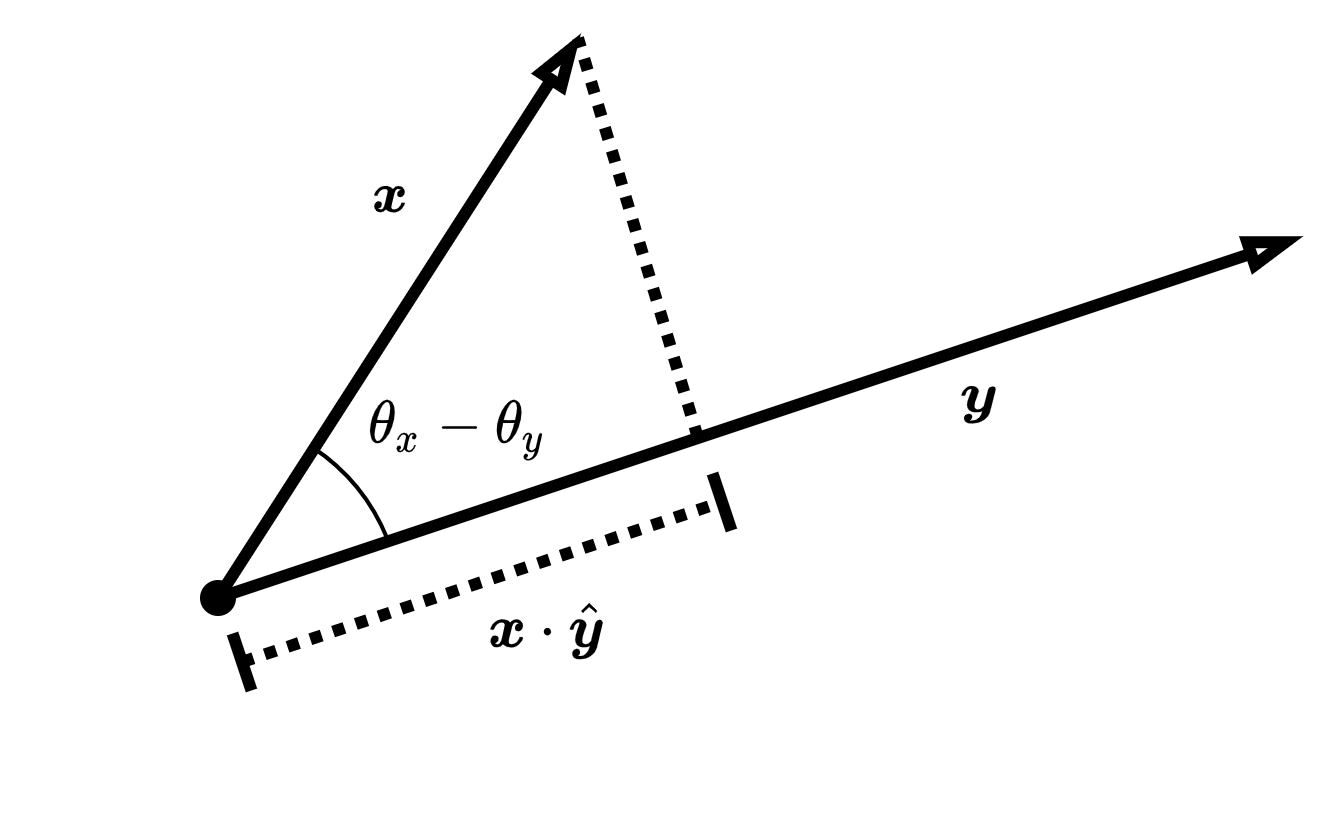
\includegraphics[scale=0.75]{dot_product.png}
	\vspace{-2em}
	\caption{Geometric meaning of the dot product}
\end{figure}\\
This generalizes to arbitrary dimension so we can always think of the dot product as a sort of projection of one vector onto another. The angle between two vectors, even when they are complex, can then always be computed as 
$$ |\theta_x - \theta_y| = \arccos(\frac{\t{Re}\{\*x\cdot\*y\}}{\|\*x\|\|\*y\|}) $$
where $\t{Re}\{\cdot\}$ denotes the real part of a complex number. This leads us to consider a special case when $\*x$ and $\*y$ are perpendicular. When the vectors differ in direction by $90^\circ$, the dot product clearly becomes zero. In the context of linear algebra, we say that two perpendicular vectors are \textbf{orthogonal}.
\definition{Orthogonality}{In an inner product space $V$, vectors $\*x$ and $\*y$ are said to be orthogonal with respect to the inner product if
$$ \langle \*x,\*y\rangle = 0 $$}
As a simple example, consider the standard basis vectors $\*e_1=\tiny\begin{pmatrix}1\\0\end{pmatrix}$ and $\*e_2=\tiny\begin{pmatrix}0\\1\end{pmatrix}$. Their dot product is clearly
$ \*e_1\cdot\*e_2 = 0$ as expected making them orthogonal. 


\newpage

\section{Changing Basis}

\subsection{Change of Basis Formula}

In many applications, we will find that the most obvious choice of basis is rarely the most convenient one. In data science and signal processing, the initial basis we have our data represented in almost always obfuscates our interpretation of the data. A simple change of basis can do wonders in elucidating patterns in data. In computational geometry, algorithms can be implemented much more efficiently if the right basis is chosen at the outset. These types of considerations (to be made clearer in the Applications section at the end of these notes) motivate the need for an ability to change basis.

Suppose are working with an $n$-dimensional vector space $V$ with initial basis set $\{\*e_1,\dots,\*e_n\}$ and we wish to re-represent all our vectors in terms of a new basis set $\{\tilde{\*e}_1,\dots,\tilde{\*e}_n\}$. In terms of either basis, we can expand any $\*x\in V$ as
$$ \*x = \underbrace{x_1\*e_1 + \dots + x_n\*e_n}_{\t{old basis}} = \underbrace{\tilde{x}_1\tilde{\*e}_1 + \dots + \tilde{x}_n\tilde{\*e}_n}_{\t{new basis}}
$$
In the original (old) basis, $\*x$ has coordinates $x_1,\dots, x_n$ while in the new basis, it has coordinates $\tilde{x}_1,\dots,\tilde{x}_n$. More explicitly, we can write
$$\*x_\t{old}=\begin{pmatrix}
	x_1 \\
	\vdots \\
	x_n
\end{pmatrix} \qquad\qquad\qquad\*x_\t{new}=\begin{pmatrix}
	\tilde{x}_1 \\
	\vdots \\
	\tilde{x}_n
\end{pmatrix}$$
We seek a formula for translating from the old basis to the new one. We want to know how to \textbf{change basis}. To see how this works, suppose we are operating in the old basis so that $\*x$ and all the new basis vectors $\tilde{\*e}_i$ are represented with components in the old basis. We then seek the coefficients $\tilde{x}_1,\dots,\tilde{x}_n$ which solve the equation
$$ \*x_\t{old} = \tilde{x}_1\tilde{\*e}_1 + \dots + \tilde{x}_n\tilde{\*e}_n = \underbrace{\begin{pmatrix}
	| & & | \\
	\tilde{\*e}_1 & \dots & \tilde{\*e}_n \\
	| & & |
\end{pmatrix}}_{\tilde{E}}\begin{pmatrix}
	\tilde{x}_1 \\
	\vdots \\
	\tilde{x}_n
\end{pmatrix} $$
As indicated in the second equality, we can cast this equation in terms of an $n\times n$ matrix $\tilde{E}=(\tilde{\*e}_1, \dots, \tilde{\*e}_n)$. So $\tilde{E}$ has the new basis vectors has its columns and we write $\*x_\t{old} = \tilde{E}\*x_\t{new}$. Since the $\tilde{\*e}_i$ form a basis, they are linearly independent and therefore there exists an inverse matrix $\tilde{E}^{-1}$. Acting with the inverse on both sides, we derive the \textbf{change of basis formula}:
$$ \*x_\t{new} = \tilde{E}^{-1}\*x_\t{old} $$
This formula tells us how to translate a vector $\*x$ represented in the old basis ($\*x_\t{old}$) into a new representation in terms of the new basis ($\*x_\t{new}$). 

\subsection{Square Matrices in a New Basis}


Consider an $n\times n$ matrix $A$ which acts on vectors $\*x\in V$ in the old basis as $\*y_\t{old}=A_\t{old}\*x_\t{old}$. If we re-represent all our vectors in terms of the new basis $\{\tilde{\*e_1}, \dots, \tilde{\*e}_n\}$, then the original form $A_\t{old}$ will no longer work as we expect it to. Indeed $A_\t{old}$ takes $\*x_\t{old}\mapsto \*y_\t{old}$, but we need a new representation $A_\t{new}$ which takes $\*x_\t{new}\mapsto \*y_\t{new}$. The old and new vectors are fundamentally the \emph{same} geometric objects after all. To represent $A_\t{old}$ in a new basis, we will write the old vectors in terms of the new ones with $\*x_\t{old}=\tilde{E}\*x_\t{new}$. Applying this, we have
\begin{align*}
	\*y_\t{old} &=  A_\t{old}\*x_\t{old}\\
	\tilde{E}\*y_\t{new} &= A_\t{old}\tilde{E}\*x_\t{new}
\end{align*}
Applying the inverse $\tilde{E}^{-1}$, we arrive at the form which maps $\*x_\t{new}\mapsto \*y_\t{new}$:
$$ \*y_\t{new} = \underbrace{\tilde{E}^{-1}A_\t{old}\tilde{E}}_{A_\t{new}}\*x_\t{new} $$
From this we can see that the matrix $A$ acts in the new basis as the transformed matrix $A_\t{new}$ given by
$$ A_\t{new} = \tilde{E}^{-1}A_\t{old}\tilde{E} $$
With this, we have a complete characterization of how to change basis:

\definition{Change of Basis}{To change basis to a new basis set $\{\tilde{\*e}_1,\dots,\tilde{\*e}_n\}$, we construct the matrix
$$ \tilde{E} = \begin{pmatrix}
	| & & | \\
	\tilde{\*e}_1 & \dots & \tilde{\*e}_n \\
	| & & |
\end{pmatrix} $$
where each new basis vector is represented here in the old basis: $\tilde{\*e}_i=\tilde{\*e}_{i,\t{old}}$. Vectors are converted from their representation in the old basis $\*x_\t{old}$ to their representation in the new basis $\*x_\t{new}$ with 
$$ \*x_\t{new} = \tilde{E}^{-1}\*x_\t{old} $$
Square matrices acting in the old basis as $A_\t{old}$ are converted to their representation in the new basis $A_\t{new}$ with
$$ A_\t{new} = \tilde{E}^{-1}A_\t{old}\tilde{E} $$}

\subsection{Rectangular Matrices in a New Basis}

Consider an $m\times n$ matrix $A$. Such a matrix represents a linear map from $\mathbb{R}^n$ to $\mathbb{R}^m$, two spaces which for $m\neq n$ have different dimension and therefore different bases. In this case, we must handle two separate basis sets --- one for the domain $\mathbb{R}^n$ and one for the codomain $\mathbb{R}^m$. To begin, for $\*x\in\mathbb{R}^n$, we have
$$ \*y = A\*x \in \mathbb{R}^m $$
As has been established, changing basis in the domain  looks like $\*x_\t{new}= \tilde{E}_n^{-1}\*x_\t{old}$ and changing basis in the codomain looks like $\*y_\t{new}=\tilde{E}_m^{-1}\*y_\t{old}$. With this, we can write
$$ \*y_\t{new}=\tilde{E}_m^{-1}A\*x_\t{old} = \tilde{E}_m^{-1}A\tilde{E}_n\*x_\t{new} $$
So then with the change of basis matrices $\tilde{E}_n$ and $\tilde{E}_m$ for $\mathbb{R}^n$ and $\mathbb{R}^m$ respectively, the $m\times n$ matrix $A$ transforms as $A_\t{new} = \tilde{E}_m^{-1}A_\t{old}\tilde{E}_n$.
 
 

\section{Dual Spaces \& Adjoint Maps}

\subsection{Linear Transformations as Vectors}

\sidenote{This section is slightly more abstract. If only interested in practical linear algebra, the main take away is the definition of the transpose and adjoint of a matrix.}
If $V$ and $W$ are vector spaces, then consider the set of all linear transformations $V\to W$, call it $\mathscr{L}(V,W)$:
$$ \mathscr{L}(V,W) \equiv \{ \t{all linear transformations } f:V\to W \} $$
It is easy to show that this space is in fact a vector space all its own. To see it, suppose we have two linear maps $f,g\in\mathscr{L}(V,W)$. Any linear combination $\*x\mapsto af(\*x) + bg(\*x)$ is also linear and therefore also lives in $\mathscr{L}(V,W)$. The zero vector in this space is the map $f_0$ which takes every vector in $V$ to $\*0\in W$. If $V$ and $W$ have respective dimensions $n$ and $m$, then every element of this space has a matrix representation which is $m\times n$. This goes to show that $\mathscr{L}(V,W)$ can be viewed as the space of all $m\times n$ matrices and that even matrices can be understood as vectors.

\subsection{Linear Functionals \& Dual Space}

Vectors are conventionally written as \emph{column vectors}, but \textbf{row vectors} also play an important role in linear algebra. In fact they arise naturally as linear transformations $\varphi:V\to\mathbb{C}$. Linear maps from a vector space to their underlying field ($\mathbb{R}$ or $\mathbb{C})$ like this are known as \textbf{linear functionals}. 
\definition{Linear Functional}{For a vector space $V$ over field $\mathbb{K}$ ($\mathbb{R}$ or $\mathbb{C}$), a linear functional on $V$ is a linear map from $V$ to its underlying field, i.e. a map $\varphi:V\to\mathbb{K}$.}
As shown in the last section, they form a vector space $\mathscr{L}(V, \mathbb{K})$ which we will denote with the special name $V^*$:
$$V^*\equiv \mathscr{L}(V,\mathbb{K})$$ 
If $V$ is $n$-dimensional, these linear functionals have $1\times n$ matrix representations which look like 
$$ \begin{pmatrix}
	\varphi_1 & \varphi_2 & \dots & \varphi_n
\end{pmatrix} \in V^* $$
This is exactly a row vector which we will denote by $\*\varphi^\t{T}$. The superscript $^\t{T}$ denotes the \emph{transpose} operation which will be defined more precisely soon. But for now it will just be used to indicate that $\*\varphi^\t{T}$ lives in $V^*$.

As vector spaces all their own, we can study linear transformations between row vector spaces. Of course, the linear transformations will have matrix representations, but consider for a moment what that must look like. If $V^*$ and $W^*$ have respective dimensions $n$ and $m$, then a linear transformation $V^*\to W^*$ must map $1\times n$ row vectors to $1\times m$ row vectors. What shape matrix does this? There is only one way to do this --- schematically we must have 
$$ [1\times n]\;[n\times m] = [1\times m] $$
Linear transformations between these spaces must be represented by $n\times m$ matrices and, crucially, they \textbf{act from the right}! So the linear transformation with matrix $B$ looks like $\*\psi^\t{T}=\*\phi^\t{T}B$.

With this knowledge in hand, consider now what linear functionals on $V^*$ look like. These are linear maps $V^*\to\mathbb{K}$ and since $\mathbb{K}$ is $1$-dimensional, the matrix representation must have size $n\times 1$. But this is just a column vector just like the elements of $V$! This illustrates a \textbf{duality} between the space $V$ and $V^*$. If we call $V^*$ the \textbf{dual space} of $V$, then we have just shown that the \emph{dual space of the dual space} is just the original space $V$. So $V$ and $V^*$ are related to each other in a symmetric way.

\definition{Dual Space}{A vector space $V$ over field $\mathbb{K}$ has a dual space $V^*$ defined by
$$ V^* = \{ \t{all linear functionals }  V \to\mathbb{K}\} $$
The dual space of the dual space $V^{**} = \{\t{all linear functionals } V^*\to\mathbb{K}\}$ can be identified with the original space: $V^{**}\cong V$. In this sense, $V$ and $V^*$ are dual to each other.
\begin{center}
	\vspace{0.5em}
	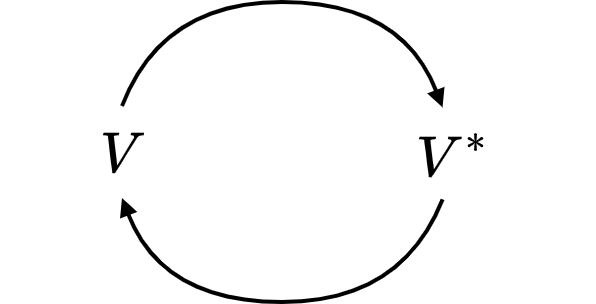
\includegraphics[scale=0.7]{dual_space.png}
\end{center}
}


\subsection{Transpose}

A linear functional $\*\varphi^\t{T}\in V^*$ acts on a vector $\*y\in V$ as $\*\varphi^\t{T}\*y$. Now suppose that we compose this with a linear transformation $U\to V$ for some other vector space $U$. That is, consider a linear transformation $U\to V$ with matrix representation $A$ so that we may write $\*y=A\*x$. The action of $\*\varphi^\t{T}$ is then $ \*\varphi^\t{T}A\*x $, which by the associativity of matrix multiplication can be computed as $(\*\varphi^\t{T}A)\*x$. From this point of view, we can identify the matrix $\*\psi^\t{T}=\*\varphi^\t{T}A$ as a linear functional belonging to the dual space $U^*$ which has components computed as
$$ \psi^\t{T}_i = \phi^\t{T}_jA_{ji} $$
So when $A$ acts from the right, matrix multiplication sums over $A$'s rows rather than its columns. This motivates the definition for the \textbf{transpose of a matrix}.
\definition{Transpose}{The transpose of an $m\times n$ matrix $A$ is an $n\times m$ matrix $A^\t{T}$ defined by
$$ A^\t{T}_{ij} = A_{ji} $$}
More explicitly, transposition reshapes a matrix so its columns become its rows:
$$ \begin{pmatrix}
	| & & | \\
	\*A_1 & \dots & \*A_n \\
	| & & |
\end{pmatrix}^\t{T} = \begin{pmatrix}
\mbox{---}\:\*A_1 \:\mbox{---}\\
\vdots \\
\mbox{---}\:\*A_n \:\mbox{---}
\end{pmatrix} $$
For vectors, the transpose operation maps $\*x \mapsto \*x^\t{T}$ where $\*x^\t{T}$ is the row vector which has the same components as the column vector $\*x$. And conversely, dual vectors are mapped under the transpose operation to column vectors: $(\*x^\t{T})^\t{T}=\*x$. When we take the transpose of a linearly transformed vector, we find 
$$(A\*x)^\t{T}=\*x^\t{T}\*A^\t{T}$$

\subsection{Adjoint/Hermitian Conjugate}

One might observe that the action of a dual vector $\*x^\t{T}\in V^*$ on a vector $\*y\in V$ looks very similar to the dot product:
$$ \*x^\t{T}\*y = x_1y_1 + \dots + x_ny_n$$
For real vector spaces, this \emph{is} identically the dot product $\*x\cdot\*y$, but for complex vector spaces, this is missing the complex conjugation: $\langle\*x,\*y\rangle = x_1^*y_1 + \dots + x_n^*y_n$. This motivates the definition of the \textbf{conjugate transpose}, which we will denote with a dagger\footnote{In engineering literature, the Hermitian conjugate is often denoted by a superscript H as $\*x^\t{H}$. The dagger is more typical in physics and functional analysis.} $\*x^\dagger$:
$$ \*x^\dagger = (\*x^*)^\t{T} $$
The conjugate transpose does exactly as the name suggests --- it takes the complex conjugate of the vector's components and then the transpose. So $\*x^\dagger$ lives in the dual space $V^*$ and now, importantly, is identical to a dot product:
$$ \*x^\dagger\*y = \langle \*x,\*y\rangle $$
This fairly mundane observation is an illustration of the \textbf{Riesz representation theorem} which states in a more abstract setting that for every linear functional $\varphi \in V^*$, there is a vector $\*v$ in $V$ such that $\varphi(\cdot) = \langle \*v,\cdot\rangle$. Namely, the action of the dual vector $\*x^\dagger$ is equivalent to a dot product with $\*x$.

There is a closely related concept called the \textbf{adjoint} of a linear transformation. The adjoint of $A$, denoted again with a dagger $A^\dagger$, is defined on general inner product spaces as that transformation which acts on the dual space such that
$$ \langle \*x,A\*y\rangle = \langle A^\dagger\*x,\*y \rangle $$
For the dot product, this is leads us to conclude that the adjoint matrix is simply the Hermitian conjugate. Consequently, these terms are often treated as synonymous, but in more general contexts in functional analysis. The adjoint is not always so simply determined. 
\definition{Hermitian Conjugate}{The Hermitian conjugate, or conjugate transpose or adjoint, of a matrix $A$ is denoted and defined by
$$ A^\dagger = (A^*)^\t{T} $$}




\newpage
\section{The Determinant}


\subsection{Visualizing Linear Transformations}


This chapter is primarily dedicated to the \emph{determinant}, a function of central importance in linear algebra. But to fully understand its meaning, it is worth looking close at linear transformations on $\mathbb{R}^2$. In this intuitive setting, the determinant can be motivated and then generalized to higher dimensions.


\begin{figure}[b]
	\centering
	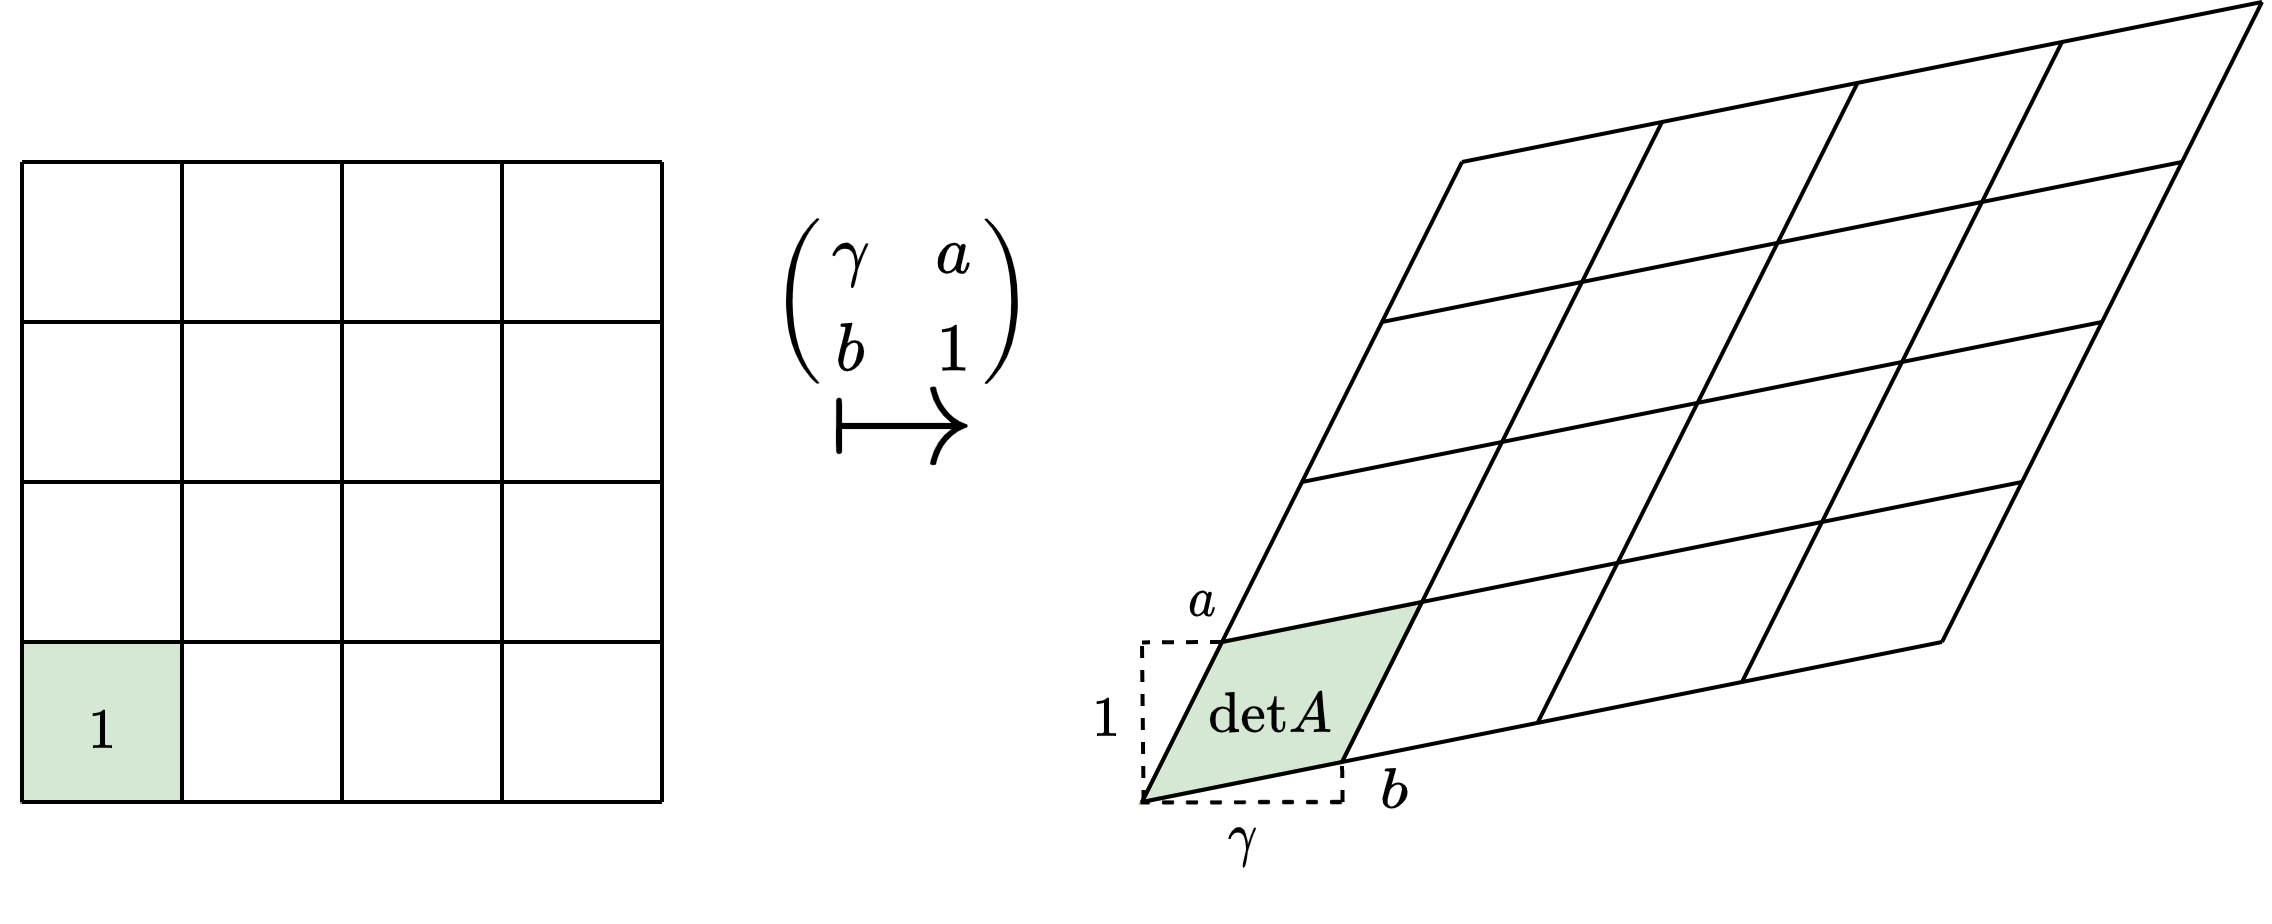
\includegraphics[scale=0.6]{determinant.png}
	\caption{\small A linear transformation on $\mathbb{R}^2$. The diagonal elements of the matrix simply scale the basis vectors while the off-diagonal elements shear the space. The determinant measures the change in area of the unit-square.}
\end{figure}

To visualize linear transformations, it must be emphasized that they fundamentally \emph{act on basis vectors}. Consider a linear transformation on $\mathbb{R}^2\to\mathbb{R}^2$, call it $A$. An arbitrary vector $\*x\in\mathbb{R}^2$ is represented in the standard basis as $\*x=x_1\*e_1 + x_2\*e_2$ so the action of $A$ looks like
$$ A\*x=A(x_1\*e_1 + x_2\*e_2) = x_1A\*e_1 + x_2A\*e_2  $$
Before the transformation, the vector $\*x$ was $x_1$ units along $\*e_1$ and $x_2$ units along $\*e_2$. After the transformation, it is $x_1$ units along $A\*e_1$ and $x_2$ units along $A\*e_2$. So the basis vectors have effectively been replaced by their transformed versions $A\*e_1$ and $A\*e_2$.  Now suppose $A$ has the form
$$  A = \begin{pmatrix}
	\gamma & a \\ b & 1
\end{pmatrix}$$
for real parameters $a,b,\gamma\in\mathbb{R}$. Up to an overall scaling, this is a completely general linear transformation $\mathbb{R}^2\to\mathbb{R}^2$. The transformed basis vectors in this case are
$$ A\*e_1 = \begin{pmatrix}
	\gamma\\b
\end{pmatrix}\qquad\qquad\qquad 
A\*e_2 = \begin{pmatrix}
	a \\ 1
\end{pmatrix} $$
The effect of this is illustrated in Figure 3 at the bottom of this page. The grid generated by $\*e_1$ and $\*e_2$ is stretched and sheared such that the new grid-generating vectors are the columns of $A$. This is what linear transformations look like.

Notice that the off-diagonal elements $a$ and $b$ are responsible for the \emph{shearing} effect of $A$. If we had $a=b=0$, then the transformation would simply scale $\*e_1\mapsto \gamma\*e_1$. As $a$ and $b$ become larger, clearly the grid transforms, becoming increasingly narrow. Eventually when $a=\gamma$ and $b=1$, the grid is squeezed to a single line and so the area (determinant) is zero. In fact, observe that these conditions are exactly when $A\*e_1=A\*e_2$, or in other words, the columns of $A$ are identical.

Observe that as a consequence of the transformation, the unit-area square in the original grid is transformed into a parallelogram which has a different area. This change in area is precisely what the determinant aims to measure. 

\begin{figure}[b!]
	\centering
	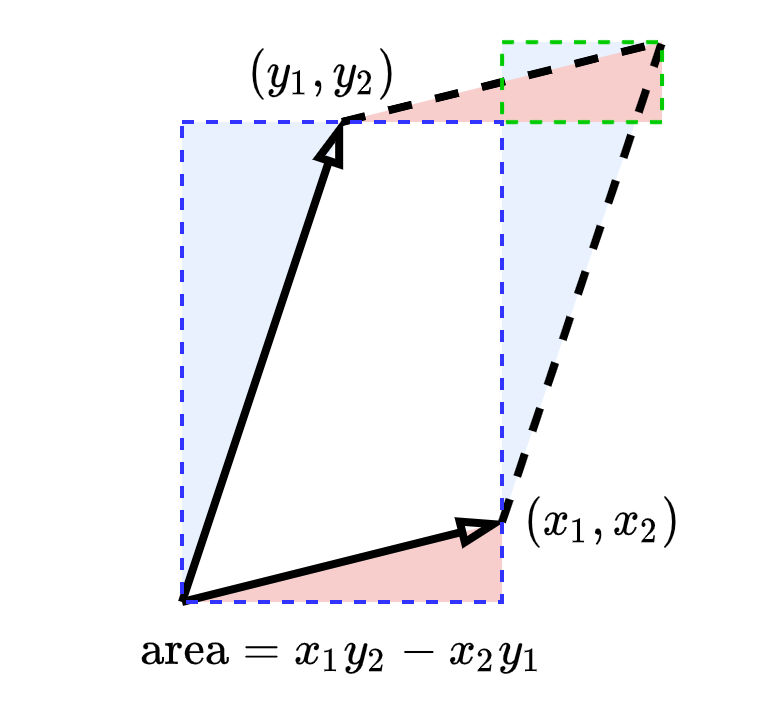
\includegraphics[scale=1]{cross_product_geometry.png}
	\caption{\small{The area of the parallelogram spanned by vectors $\*x=(x_1,x_2)$ and $\*y=(y_1,y_2)$ is computed by the cross product $|\*x\times\*y| = x_1y_2 - x_2y_1$. The first term $x_1y_2$ is the area of the blue-dashed rectangle which contains the red and blue triangles. When the red and blue triangles are translated to the upper-right corner of the parallelogram, they cover the remainder of the parallelogram, but there is some extra area that must be subtracted off. This is exactly the second term $x_2y_1$, the area of the green-dashed rectangle.}}
\end{figure}

\newpage
\subsection{The Determinant}

\sidenote{To paint a complete picture of the determinant, the abstract approach is taken and we derive its functional form. For this, it helps to have some familiarity with permutations.}
\definition{Determinant}{The determinant of an $n\times n$ matrix $A=(\*A_1, \dots, \*A_n)$ is a function with the following properties:
\begin{itemize}
	\setlength\itemsep{-0.1em}
	\item Identity: $\det\mathbbm{1}= 1$
	\item Multilinear: $\det( \*A_1,\dots,\sum_ia_i\*e_i, \dots, \*A_n)  = \sum_ia_i \det( \*A_1,\dots,\*e_i,\dots,\*A_n) $
	\item Alternating: $\det( \*A_1,\dots, \*v,\dots,\*v,\dots,\*A_n)  = 0$
\end{itemize}}
Expanding each column vector in the standard basis as $\*A_i = \sum_jA_{ji}\*e_j$, the multilinear property of the determinant allows us to decompose $\det A$ as
\begin{align*} 
	\det A &= \det(\sum_{j_1}A_{j_11}\*e_{j_1}, \dots, \sum_{j_n}A_{j_nn}\*e_{j_n})  = \sum_{j_1}\dots\sum_{j_n}A_{j_11}\dots A_{j_nn}\det(\*e_{j_1}, \dots,\*e_{j_n})
\end{align*}
There are $n$ sums which each run over all $n$ basis vectors leading to a whopping total of $n^n$ terms in this sum. However, things are greatly simplified by the alternating property which dictates that the only non-zero terms are those with distinct values for $j_1,\dots,j_n$. This is equivalent to summing over every permutation of $j_1,\dots,j_n$ (of which there are $n!$). The set of all permutations of $n$ elements is known as the \textbf{symmetric group} of degree $n$ and we denote it by $S_n$. Each permutation $\sigma$ is a reordering of the $n$ values: $(1,2,\dots,n) \mapsto (\sigma(1),\sigma(2),\dots,\sigma(n))$. With this, we can write
$$ \det A = \sum_{\sigma\in S_n}A_{\sigma(1)1}\dots A_{\sigma(n)n} \underbrace{\det(\*e_{\sigma(1)},\dots,\*e_{\sigma(n)})}_{\pm 1} $$
As indicated, the determinant over the basis vectors is either $1$ or $-1$ depending on the permutation. Since $(\*e_1,\dots,\*e_n)=\mathbbm{1}$, the determinant of the unpermuted basis vectors is $1$. Then the alternating property dictates that any \textbf{odd permutation}\footnote{An even (odd) permutation is one which is equivalent to an even (odd) number of pairwise swaps.} of the basis vectors must have determinant $-1$ and any \textbf{even permutation} will have determinant $1$. This distinction is encoded in the \textbf{sign of a permutation}, denoted $\t{sgn}(\sigma)$. With this, we arrive at an explicit formula for the determinant of a matrix:
$$ \det A = \sum_{\sigma\in S_n} \t{sgn}(\sigma) A_{\sigma(1)1}\dots A_{\sigma(n)n} $$
Observe how we arrived at the form of this function purely from the three properties in the definition. This proves that there is in fact only one \textbf{unique} function which has these three properties. That is why we call it \emph{the} determinant rather than \emph{a} determinant.

Consider the simple example of a $2\times 2$ matrix. The sum is over all permutations of $\{1,2\}$ of which there are only 2: $\{1,2\}$ and $\{2,1\}$. The above formula then gives
$$ A = \begin{pmatrix}
	A_{11} & A_{12} \\
	A_{21} & A_{22}
\end{pmatrix} \quad\implies \quad \det A =A_{11}A_{22} - A_{21}A_{12} $$
which aligns with the cross product formula from the previous section. As another example, consider a $3\times 3$ matrix. Now the sum is over all permutations of $\{1,2,3\}$ of which there are $3!=6$. The even permutations are are $ \{1,2,3\} \:\: \{2,3,1\}\:\:\{3,1,2\}$ and the odd permutations are $ \{1,3,2\}\:\: \{2,1,3\}\:\:\{3,2,1\} $.
so the determinant formula gives
\begin{multline*}
	A=\begin{pmatrix}
	A_{11}&A_{12}&A_{13} \\
	A_{21}&A_{22}&A_{23}\\
	A_{31}&A_{32}&A_{33}
	\end{pmatrix}
 \quad\implies\quad \det A = A_{11}A_{22}A_{33} + A_{21}A_{32}A_{13} + A_{31}A_{12}A_{23} \\ - A_{11}A_{32}A_{23} - A_{21}A_{12}A_{33} - A_{31}A_{22}A_{13}
\end{multline*}






\subsection{Properties of The Determinant}




\newpage

\section{Types of Square Matrices}


\subsection{Singular Matrices}

Perhaps the most important general classification of matrices is singular vs. non-singular. T
\definition{Singular Matrix}{A square matrix $A$ is called singular if it has linearly dependent columns/rows. This is equivalent to all of the following conditions:
\begin{itemize}
	\setlength\itemsep{0.01em}
	\item $\det A = 0$
	\item $A\*x=\*0$ for some $\*x\neq\*0$ (i.e. $\t{null}(A)$ is nontrivial)
	\item $A^{-1}$ does not exist
\end{itemize}}

\subsection{Projection Matrices}

\definition{Projection Matrix}{A square matrix $A$ is called a projection matrix if it satisfies the \textbf{idempotence} condition:
$$ A^2=A $$}

\subsection{Orthogonal Matrices}

\definition{Orthogonal Matrix}{A square matrix $A$ is called orthogonal if its columns are orthonormal vectors. This is equivalent to the condition that the transpose $A^\t{T}$ is the inverse $A^{-1}$:
$$ A^\t{T}A=\mathbbm{1} $$}

\subsection{Rotation Matrices}

\definition{Rotation Matrix}{A square matrix $A$ is called a rotation matrix if it is an orthogonal matrix with determinant 1:
$$ A^\t{T}A=\mathbbm{1} \qquad\qquad\qquad \det A = 1 $$}

\subsection{Symmetric \& Hermitian Matrices}


\definition{Symmetric Matrix}{A square matrix is called symmetric if it is equal to its transpose:
	$$ A^\t{T} = A $$}

\definition{Hermitian Matrix}{A square matrix is called Hermitian if it is equal to its conjugate transpose:
$$ A^\dagger = A $$}

\subsection{Positive Definite Matrices}




\newpage
\section{Matrix Decompositions}

\subsection{Motivation}

To effectively apply linear algebra, it is important to be familiar with different ways to decompose, or factorize, a matrix. A decomposition of a matrix $A$ is breaking into a product of other more simple matrices $F_i$ so that $A=\prod_i F_i$. In all the matrix decomposition methods that will be reviewed in this chapter, they use either two factors $A=F_1F_2$ or three factors $A=F_1 F_2 F_3$. 

\subsection{Eigendecomposition}
\addcontentsline{toc}{subsection}{Eigendecomposition}
Perhaps the most important matrix factorization is known as the \textbf{eigendecomposition}. The name comes from the German word ``\emph{eigen}" which means ``\emph{own}", as in ``\emph{all its own}". As this naming suggests, the eigendecomposition is very characteristic of a given matrix. It applies to square matrices but breaks a matrix down to its most fundamental operations. It is ubiquitous in applied math. In quantum mechanics, energies are computed through an eigendecomposition. In data science, principal component analysis (PCA) is just an eigendecomposition of a covariance matrix. In dynamical systems, an eigendecomposition readily gives the solutions to an ODE. 

Suppose we have a matrix $A$ and we want to find a new basis in which $A$ takes the simplest form possible. In particular, we want $A$ to be a diagonal matrix which we will call $\Lambda$. If the basis vectors that achieve this are arranged in the columns of a matrix $V$, then the change of basis is $\Lambda = V^{-1}AV$. Rearranged for $A$, we have the eigendecomposition:
\definition{Eigendecomposition}{The eigendecomposition of a square $n\times n$ matrix $A$ is
$$ A = V\Lambda V^{-1} $$
where $\Lambda = \t{diag}(\lambda_1,\dots,\lambda_n)$ is a diagonal matrix and $V$ has columns $V=(\*v_1,\dots,\*v_n)$ such that $A\*v_i=\lambda_i\*v_i$}
We call this \textbf{diagonalizing} the matrix $A$. It remains to be shown however that such a transformation even exists for a matrix. To begin, we seek solutions to the equation
$$ A\*x = \lambda\*x $$
where $\lambda\in\mathbb{C}$ is just a scalar complex number. Geometrically, we are looking for vectors $\*x$ which are not rotated at all by $A$, but instead are only scaled by some factor $\lambda$. A solution $\*x$ is called an \textbf{eigenvector} of $A$ and the corresponding value for $\lambda$ is called an \textbf{eigenvalue}. To find solutions, we can rearrange this equation to write 
$$ (A - \lambda\mathbbm{1})\*x=\*0 $$
Evidently then our solutions must belong to the null space of a matrix $A-\lambda\mathbbm{1}$. Clearly for any matrix, $\*x=\*0$ is a solution, but we do not call this an eigenvector --- eigenvectors must be non-zero. Now depending on the value of $\lambda$, the matrix $A-\lambda\mathbbm{1}$ could be singular or non-singular. But for nontrivial solutions, we must insist that it is singular --- it must have determinant zero. Therefore we write
$$ \det(A-\lambda\mathbbm{1}) = 0 $$
This is an equation to solve for $\lambda$. If $A$ is an $n\times n$ matrix, the formula for the determinant applied above yields a \textbf{characteristic polynomial} in $\lambda$ which we now must find the roots of. Generically, the determinant unravels to
$$ a_n\lambda^n + a_{n-1}\lambda^{n-1} + \dots + a_1\lambda + a_0= 0 $$
for some set of coefficients which depend on the entries in $A$. Finding the roots of the characteristic polynomial gives the eigenvalues of $A$. All that remains is to find the eigenvectors. For this, we plug the found values for $\lambda$ back into $A\*x=\lambda\*x$. There are $n$ unknowns (the components of $\*x$) and $n$ equations so this can be solved for $\*x$.

Let's make this more concrete with an example. Consider a $2\times 2$ orthogonal matrix of the form
$$ A = \begin{pmatrix}
	a & b\\
	b & -a
\end{pmatrix} $$
The characteristic polynomial is computed as
$$ \det \begin{pmatrix}
	a-\lambda & b \\
	b & -a-\lambda
\end{pmatrix} =(\lambda-a)(\lambda+a) - b^2$$
which simplifies to $ \lambda^2 - a^2-b^2$. The roots of this polynomial are easily found giving the eigenvalue solutions:
$$ \lambda_\pm = \pm\sqrt{a^2+b^2}  $$

\subsection{Cholesky Decomposition}

The Cholesky decomposition comes in handy when working with positive-definite matrices. The idea is fairly simple. If $A$ is positive-definite, then perhaps, like with positive numbers, we can take a square root. To quickly derive the Cholesky decomposition, first write the eigendecomposition
$$ A = V\Lambda V^\t{T} $$
Now since all the eigenvalues are positive, we can define the square root matrix $\Lambda^{1/2}$ such that $\Lambda = \Lambda^{1/2}\Lambda^{1/2}$. Then we have
$$ A= (V\Lambda^{1/2})(\Lambda^{1/2}V^\t{T}) $$


\subsection{Singular Value Decomposition (SVD)}





\newpage
\section{Direct Sums \& Tensor Products}


\subsection{Combining Vector Spaces}

This chapter deals with a fairly different topic from what is covered in the rest of these notes. Here, the focus is on how the \emph{combine} vector spaces. Suppose we have two vectors spaces $U$ and $V$ which we would like to combine into one larger vector space. In general, we will work with cartesian product:
$$ U\times V \equiv \{ (\*u,\*v)\:|\:\t{for all } \*u\in U \t{ and } \*v\in V\}$$
This set contains every element of $U$ combined with every element of $V$, but it does \emph{not} yet have any algebraic structure. How do we add elements in this space? What does scalar multiplication look like? These details can be handled in different ways. The two canonical ways are through the direct sum and the tensor product.

\subsection{Direct Sum}

The direct sum of vector spaces, denoted by the symbol $\oplus$, is defined as follows
\definition{Direct Sum of Vector Spaces}{For vector spaces $U$ and $V$, the direct sum $U\oplus V$ is defined as the product $U\times V$ with vector addition and scalar multiplication operating elementwise:
$$ (\*u_1,\*v_1) + (\*u_2,\*v_2) = (\*u_1+\*u_2, \*v_1+\*v_2) $$
$$ a(\*u,\*v) = (a\*u, a\*v) $$}
This is perhaps the simplest way to combine vector spaces. Consider that if $\*e_1,\dots,\*e_n$ forms a basis of $U$ and if $\*f_1,\dots,\*f_m$ forms a basis of $V$, then there is a basis of $U\oplus V$ given by all the elements $\*e_i\oplus\*0$ and those elements $\*0\oplus\*f_j$. This implies that the direct sum has dimension
$$ \dim U\oplus V = m + n $$

\subsection{Tensor Product}

\definition{Tensor Product}{For vector spaces $U$ and $V$ with respective bases $(\*e_1,\dots,\*e_n)$ and $(\*f_1,\dots,\*f_m)$, the tensor product $U\otimes V$ can be defined as the vector space 
$$ U\otimes V \equiv \t{span}\{ \*e_i \otimes\*f_j \} $$}

\newpage
\section*{}
\addcontentsline{toc}{section}{Applications}
\vspace{2in}
\begin{center}
	\Huge{\textbf{Applications}}
\end{center}
\vspace{1in}
\rule{\textwidth}{2pt}
The remaining pages of these notes contain various applications of linear algebra. Depending on the reader's interests, some or all of these examples may not be of interest. However an attempt was made to cover a wide range of interests including statistics, machine learning, quantum computing, graph theory, and others.
\\
\rule{\textwidth}{2pt}

\newpage
\section{Statistics: PCA \& Simulation}
\subsection{Multivariate Normal Distribution}
Linear algebra is ubiquitous in statistics and data science. Whenever we work with multiple random variables, it is natural to express the statistics and probability theory in terms of vectors and matrices. Consider the normal distribution. In one variable $x\sim\mathcal{N}(\mu,\sigma^2)$, the probability density function (pdf) is $p(x)=(2\pi\sigma^2)^{-1/2} \exp{-(x-\mu)^2/2\sigma^2}$ where $\mu$ is the mean and $\sigma^2$ is the variance. When we have $n$ normal random variables $x_1,\dots, x_n$ all with different means and variances, there can also be \textbf{correlations} between them. The variables are packaged as a vector $\*x$ with mean $\*\mu$ and the variance is replaced by a \textbf{covariance matrix} $\Sigma$ where $\Sigma_{ij}$ captures the correlation between variables $x_i$ and $x_j$. So $\*x\sim\mathcal{N}(\*\mu,\Sigma)$ has multivariate normal distribution with pdf
$$ p(\*x) = \det(2\pi\Sigma)^{-1/2} \exp{ -\frac{1}{2}(\*x-\*\mu)^\t{T}\Sigma^{-1}(\*x-\*\mu) } $$


\subsection{Principal Component Analysis (PCA)}
Suppose we have a data set consisting of $n$ samples where each sample $\*x^{(i)}$ is a vector containing $m$ values/features. We can package these values into an $m\times n$ matrix $X_{ij}=x^{(j)}_i$:
$$ X = \begin{pmatrix}
	| & & |\\
	\*x^{(1)} & \dots & \*x^{(n)}\\
	| & & |
\end{pmatrix} $$
Each sample is a point in $\mathbb{R}^m$ so we can visualize the data set as $n$ points in $m$-dimensional space. The goal of PCA then is to find the directions in that space along which the data is most spread, i.e. the directions of highest variance. To do so, we will certainly need to have an estimate for the covariance matrix. From this data, the standard way to estimate the covariance matrix is 
$$ \hat{\Sigma} = \frac{1}{n-1}XX^\t{T}  $$
\begin{wrapfigure}[22]{r}{0.5\textwidth}
	\centering
	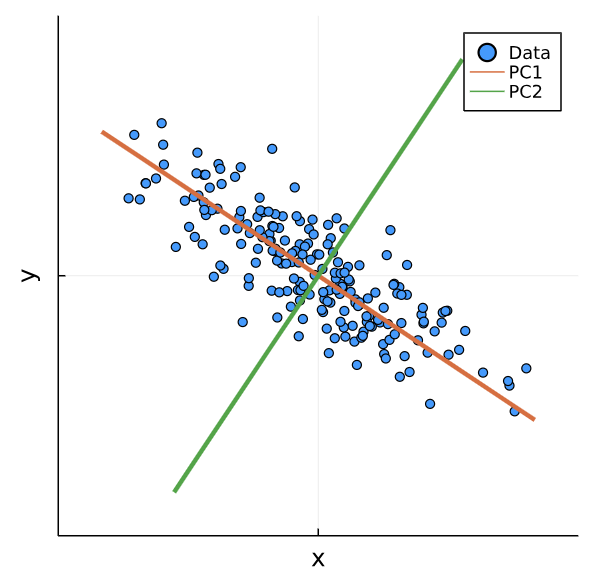
\includegraphics[scale=0.6]{pca.png}
	\caption{\small{Illustration of PCA applied to a data set of 2 features ($n=200$). The first principle component (PC1) is clearly oriented along the direction of greatest variance.}}
\end{wrapfigure}

PCA works by taking the \textbf{eigendecomposition} of the covariance matrix and then focusing on only those eigenvectors with the largest eigenvalues. Indeed, the covariance matrix is symmetric by construction and therefore has real eigenvalues which can be ordered. Moreover, it has orthogonal eigenvectors which form an orthonormal basis of $\mathbb{R}^m$. With the eigendecomposition, we can diagonalize the covariance matrix as
$$ \t{diag}(\lambda_1, \dots, \lambda_m) = V^\t{T}\hat{\Sigma}V $$

This can be understood as a simple change of basis where the new orthonormal basis of $\mathbb{R}^m$ is determined by the eigenvectors of $\hat{\Sigma}$. Indeed, transforming our data to this basis\footnote{Recall that rectangular matrices change basis as $X_\t{new}=V^{-1}X_\t{old}U$ where $V$ and $U$ are change of basis matrices for the codomain and domain respectively. Here we leave the domain basis unchanged: $U=\mathbbm{1}_n$.}, we get the new data matrix $\widetilde{X}=V^\t{T}X$. It is straight forward to verify that the estimated covariance of the transformed data is exactly the diagonalized matrix:
$$ \t{diag}(\lambda_1,\dots,\lambda_m) = \frac{1}{n-1}\widetilde{X}\widetilde{X}^\t{T} $$

We call the eigenvectors of $\hat{\Sigma}$ the \textbf{principle components} of the data. Importantly, since the new covariance matrix is diagonal, the principle components are \textbf{uncorrelated}. The eigenvalues $\lambda_1,\dots,\lambda_m$ are precisely the variances of the data along each principal component, so from the eigendecomposition, we can read off directly the directions of greatest variance --- they are simply the eigenvectors with the greatest eigenvalues.


PCA is a popular method in statistics and data science for reducing a high-dimensional data set to a lower dimensional one with a minimal loss of information. This is known as \textbf{dimensional reduction}. PCA can do this by forming a low-dimensional data set consisting of just the first few principal components of the data. 
\vspace{1em}
\subsection{Monte Carlo Simulation}
There are many scenarios where one wants to computationally \emph{generate} random data with a particular distribution. Computational methods that use randomly generated data are known as \textbf{Monte Carlo methods}. Examples include simulating stock movements for portfolio risk evaluation or simulating complex physical systems at nonzero temperature.

Every standard programming language has a library capable of generating data with a standard normal distribution\footnote{A pseudorandom number generator outputs uniformly distributed data $u\sim [0,1]$. If $F$ is the standard normal CDF, then $x= F^{-1}(u)$ is distributed as $\mathcal{N}(0,1)$}, but it is typically left up the user to transform this to have the desired mean and variance. Generally, with $x\sim\mathcal{N}(0,1)$, we can define a new variable with any mean and variance with the appropriate scaling and shift:
$$ x\sim\mathcal{N}(0,1) \quad\implies\quad \sigma x+\mu \sim \mathcal{N}(\mu,\sigma^2) $$
This is all well and good for the single variable case, but once we move to the multivariate case, it is less obvious how to generate data with an arbitrary covariance matrix. The single variable procedure can be repeated $n$ times to generate an $n\times 1$ vector $\*x\sim\mathcal{N}(0,\mathbbm{1})$. With this vector, it is possible to perform a linear transformation which produces a vector with any desired covariance matrix $\Sigma$. Since $\Sigma$ is positive semi-definite, we can always ``take a square root" and write
$$ \Sigma = LL^\t{T} $$
for some matrix $L$. For example, this could be a \textbf{Cholesky decomposition}, making $L$ a lower-triangular matrix. With $\*x\sim \mathcal{N}(\*0, \mathbbm{1})$, we can transform and shift the data to have the covariance and mean we desire:
$$\*x\sim \mathcal{N}(\*0, \mathbbm{1}) \quad\implies\quad   L\*x + \*\mu\sim \mathcal{N}(\*\mu,\Sigma)$$


\newpage
\section{Graph Theory}
\begin{wrapfigure}[12]{r}{0.33\textwidth}
	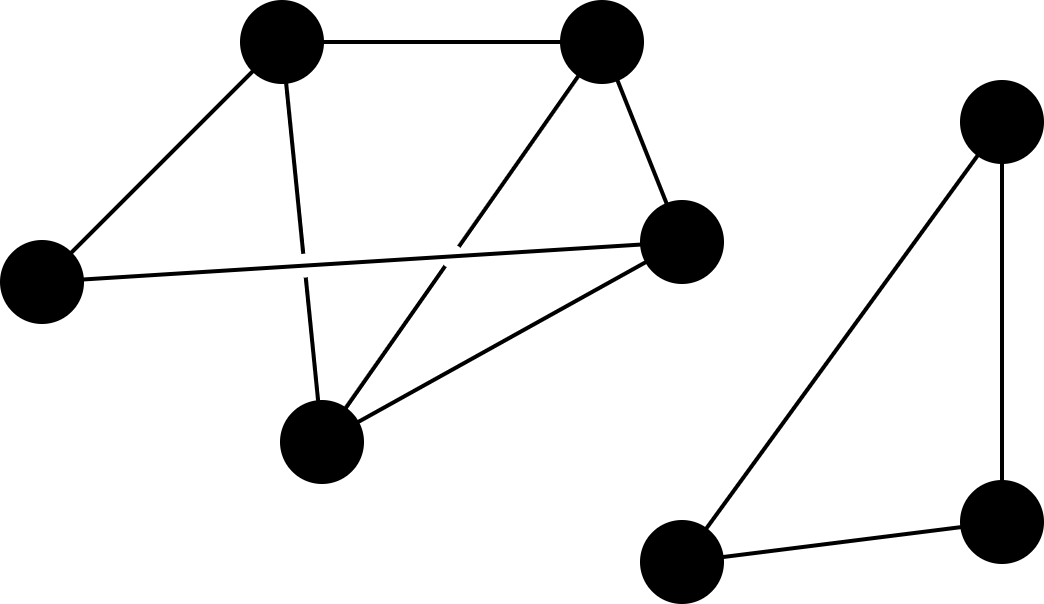
\includegraphics[scale=0.65]{graph.png}
	\caption{An undirected simple graph with 8 nodes and 2 connected components}
\end{wrapfigure}
Graph theory concerns itself with \emph{graphs}, webs of connections that can be visualized as in the figure to the right. A graph has a set of \textbf{nodes} which are connected by \textbf{edges}. In general, the edges can be \textbf{directed} so that they point from one node to another, but we will focus on the simpler case of \textbf{undirected graphs} which have edges that simply connect two nodes --- there is no direction associated with a connection. In general, a graph can also have edges which connect a node to itself (called a \textbf{loop}) or have two edges which connect the same two nodes. A graph which has no loops and no repeated edges is called a \textbf{simple graph}. We will focus on these. The precise definition we will use is
\definition{Undirected Simple Graph}{An undirected simple graph $\mathcal{G}=(V,E)$ is a set of vertices $V$, called nodes, and edges $E$ which connect the nodes: 
$$ E = \{ \{a,b\} \:|\: a,b\in V \t{ and } a\neq b\} $$}
Another useful definition is for a \textbf{connected graph}. A connected graph is one in which every pair of nodes can be connected through some sequence of edges. For example, in the graph shown in Figure 6, there are two connected subgraphs, a.k.a. connected components. In this short application note, we will ask the question:

\begin{center}
	\emph{Given an undirected simple graph $\mathcal{G}$, how many connected components does it have?}
\end{center}
To answer this question, we must build up some theory to describe graphs in terms of linear algebra. First we will define the \textbf{adjacency matrix} which will encode which nodes are connected.
\definition{Adjacency Matrix}{For undirected simple graph $\mathcal{G}$ with $n$ nodes and edge set $E$, the adjacency matrix $A$ is the $n\times n$ matrix with elements
$$ A_{ij} = \begin{cases}
	1 & \{i,j\}\in E \:\:\:\:(\t{if node }i\t{ is connected to node }j) \\
	0 & \t{otherwise} 
\end{cases} $$}
So the adjacency matrix is full of ones and zeros indicating which nodes are connected. Note that for undirected graphs, the adjacency matrix is symmetric by construction: $A^\t{T}=A$.

Next, we should define the \textbf{degree} of a node in a graph. This is defined by the number of edges incident on it. The degree of node $i$ is
$$ \t{deg}(i)=\t{number of edges in $E$ incident on node $i$} $$
With this, we can finally define the crucial ingredient we need to answer our question: the \textbf{graph Laplacian}:
\definition{Graph Laplacian}{For graph $\mathcal{G}$, the Laplacian matrix is an $n\times n$ matrix $L$ defined by
$$ L \equiv D - A $$
where $A$ is the adjacency matrix of $\mathcal{G}$ and $D$ is the degree matrix defined by
$$ D_{ij} = \begin{cases}
	\t{deg}(i) & i=j \\
	0 & \t{otherwise}
\end{cases} $$
}
A few observations. Consider that by looking at row $i$ of the adjacency matrix, we can count the number of nodes that connect to node $i$ by just counting the number of non-zero elements in the row. And since we are focusing on simple graphs with no loops or repeated edges, this number of connected nodes is the same as the number of incident edges, i.e. the degree of node $i$. Explicitly, we have
$$ \sum_j A_{ij} = \t{deg}(i) = D_{ii}$$
This implies that the sum across any row of the Laplacian matrix is zero:
$$ \sum_{j}L_{ij} =0 $$
This can be read another way. Defining the vector of ones $\*1=(1\:1\:\dots\:1)^\t{T}$, this equation tells us that $\*1$ lives in the null space of the graph Laplacian: $L\*1=\*0$. Therefore the Laplacian matrix has a nontrivial null space and is always singular. Perhaps this motivates us to look closely at $\t{null}(L)$. We seek solutions to $ L\*v=\*0 $. This can be expanded out to write
$$ \*v\in\t{null}(L) \quad \implies \quad\t{deg}(i)v_i = \sum_j A_{ij}v_j $$
Think about what the equation on the right means. Suppose we have a graph with multiple connected components. For all the nodes in connected component $\mathcal{C}$, we have to be able to write
$$ \t{deg}(i)= \sum_{j\in\mathcal{C}} A_{ij} \quad\forall i\in \mathcal{C}$$
This is, after all, essentially what it means to be a connected component. With this understanding, it can be seen that the null space of the graph Laplacian exactly tells us what the connected components of the graph are.
\definition{Number of Connected Components}{For an undirected simple graph $\mathcal{G}$, each connected component $\mathcal{C}$ corresponds to a vector $\*v$ with components
$$ v_i = \begin{cases}
	1 & \t{if node } i\in \mathcal{C} \\
	0 & \t{otherwise}
\end{cases} $$
which belongs to the null space of the graph Laplacian: $\*v \in\t{null}(L)$. Therefore the number of connected components equals the dimension of the null space of $L$:
$$ \t{number of connected components in $\mathcal{G}$} = \t{dim}(\t{null}(L)) $$}


\newpage
\section{Deep Learning}
\textbf{Machine learning} is concerned with constructing statistical models which can learn from data how to perform a task. The statistical models commonly used in machine learning include linear regression, logistic regression, decision trees, random forests, and importantly \textbf{neural networks}. Neural networks are the basic objects used in \textbf{deep learning}, a sub-field of machine learning that focuses on models with a high number of parameters. They are statistical models that are loosely inspired by the structure of the human brain. Just as signals are passed through the brain, activating certain neurons along the way, neural networks pass data through multiple layers ``activating" certain components along the way.
\definition{Feed-Forward Neural Network}{A feed-forward neural network $\mathscr{N}$ consists of $L$ sequential layers. Each layer is a function of the form $\mathcal{L}^{(n)} = \sigma^{(n)}\circ f^{(n)}$ where $\sigma^{(n)}$ is a nonlinear function and $f^{(n)}$ is an affine transformation. The network is the composition of $L$ layers:
$$\mathscr{N} = \mathcal{L}^{(L)}\circ \dots \circ \mathcal{L}^{(1)}$$
If the output of layer $n$ is denoted $\*x^{(n)}=\mathcal{L}^{(n)}(\*x^{(n-1)})$, then the network can be succinctly written
$$ \*x^{(n)} = \sigma^{(n)}\left( W^{(n)}\*x^{(n-1)} + \*b^{(n)}\right) $$
where $W^{(n)}$ is a matrix of weights and $\*b^{(n)}$ is a bias vector.}
The nonlinear functions $\sigma$ are called \textbf{activation functions} and they are key to deep learning. Without a nonlinear function between each layer, the entire network would always be fully equivalent to one single layer. This is true because the composition of affine maps is always just another affine map. So without activation functions, neural networks would just be a highly inefficient way to evaluate a single affine transformation. Some common activation functions include
\begin{align*}
	 \sigma(x) = \frac{1}{1+e^{-x}} && \tanh(x)=\frac{e^{x} - e^{-x}}{e^{x} + e^{-x}} && \t{reLu}(x)=\begin{cases}
		x & x>0 \\
		0 & \t{otherwise}
	\end{cases}
\end{align*}
respectively known as the sigmoid function (or logistic function), hyperbolic tangent (or ``tanch"), and the rectified linear unit (or ``rel-U"). Perhaps the primary reason to choose one activation function over another is their output range. The sigmoid function has output on $[0,1]$, the tanh function has output on $[-1,1]$, and the $\t{reLu}$ function has output on $[0,\infty]$. Depending on what kind of information the model is supposed to handle, it may or may not make sense to allow negative values or arbitrarily large values.

Once the model architecture is decided on, the neural network must be \textbf{trained} on a data set so that the model parameters are tuned to work as they ought to. We must decide on a \textbf{loss function} which measures the error in the network output. Then we tune the parameters of the model so as to minimize the loss function. A standard choice of loss function is the \textbf{mean square error} (MSE). For $N_\t{train}$ data points to train on, the MSE can be computed using the known true value $\*y_i$ for each data point and the estimated value from the network $\hat{\*y}_i$:
$$ \t{MSE} = \frac{1}{2N_\t{train}}\sum_{i=1}^{N_\t{train}}\|\hat{\*y}_i - \*y_i\|_2^2 $$
where $\|\cdot\|_2$ denotes the $\ell^2$-norm. The factor of $1/2$ out front is conventional and simply cleans up a factor of 2 that we would otherwise have to carry around in the minimization procedure.

\subsection{Convolutional Neural Networks (CNNs)}
There is a special type of neural network where the affine transformation between layers is a \textbf{convolution}. The convolution of two vectors is given by
$$ (\*x * \*y)_i = \sum_jx_{j-i}y_j $$




\newpage
\section{Ordinary Differential Equations (ODEs)}
An \textbf{ordinary differential equation} (ODE) is an equation of the form
$$ u^{(n)} + a_{n-1}u^{(n-1)} + \dots + a_2u'' + a_1u' + a_0u + b = 0 $$
for some set of $t$-dependent coefficients $a_0,\dots,a_{n-1}$ and $b$. As written, this is an \textbf{$\*n^\t{th}$ order equation} since the highest derivative is the $n^\t{th}$. This can be recast into a vectorial equation of degree 1 by defining $u_{i+1} = u_i'$ with base case $u_0=u$. Then the above ODE can be written as the system of equations
\begin{align*}
	u_0' &= u_1 \\
	u_1' &= u_2 \\
	\vdots &\\
	u_{n-2}' &= u_{n-1}\\
	u_{n-1}' &= -a_0u_0 - a_1u_1 -\dots -a_{n-1}u_{n-1} - b
\end{align*}
This can of course be recast as a matrix equation with the vector $\*u=(u_0\:u_1\:\dots\:u_{n-1})$ and a matrix $A$ so that
$$ \*u' = A\*u + \*b $$


\newpage
\section{Quantum Computing}
Quantum mechanics is fundamentally a linear theory. Physical systems are described by a vector in a Hilbert space which we will call $\mathscr{H}$. Vectors in this space are conventionally denoted using \textbf{Dirac notation}, or \textbf{bra-ket notation}:
$$\ket{\psi} \in \mathscr{H}$$
This notation is fairly natural when one realizes that it comes from taking inner products. Instead of writing inner products as $\langle\cdot,\cdot\rangle$, physicists write $\bra{\cdot}\ket{\cdot}$. This is viewed as a dual vector (bra) $\bra{\cdot}$ acting on a vector (ket) $\ket{\cdot}$\footnote{Thanks to the Riesz representation theorem, inner products can always be viewed this way.}. One nice property of Dirac notation is it neatly allows us to label vectors however we like. We can replace the dot in $\ket{\cdot}$ with anything descriptive and write $\ket{\t{descriptive label}}$.

To get into some detail about how quantum mechanics work and what quantum computers do, we must first establish a basic form of the postulates of QM:
\definition{Posulates of Quantum Mechanics}{
\begin{itemize}
	\setlength\itemsep{0.1em}
	\item The state of a physical system is totally specified by a \textbf{state vector} $\ket{\psi}\in\mathscr{H}$
	\item Every measurable property corresponds to a Hermitian linear operator $A:\mathscr{H}\to\mathscr{H}$
	\item When a measurement is made, the only observed values are the eigenvalues of the corresponding operator, i.e. those $\lambda\in\mathbb{R}$ such that $A\ket{\lambda}=\lambda\ket{\lambda}$
	\item Immediately after measuring value $\lambda$, the system is in an eigenstate $\ket{\lambda}$	
	\item For a physical system in state $\ket{\psi}$, the probability of measuring value $\lambda$ is $\abs{\bra{\lambda}\ket{\psi}}^2$
	\item State vectors evolve in time via a unitary transformation: $\ket{\psi(t)}=U(t)\ket{\psi(0)}$
\end{itemize}}
To the uninitiated, these postulates will surely look bizarre. But, simply put, they work. We could ask endless questions about the picture of nature that is painted by quantum mechanics, but ultimately we can only care about what we measure. And since the postulates provide a perfectly well formulated way to predict measurement probabilities, we will move forward to get to the operational details without getting bogged down in the philosophical quagmire. 

The simplest possible quantum system also happens to be the fundamental object in quantum computing: the \textbf{qubit}. So talking about qubits will serve as both a basic introduction to quantum mechanics and as an introduction to quantum computing. 

\begin{wrapfigure}{r}{0.5\textwidth}
	\centering
	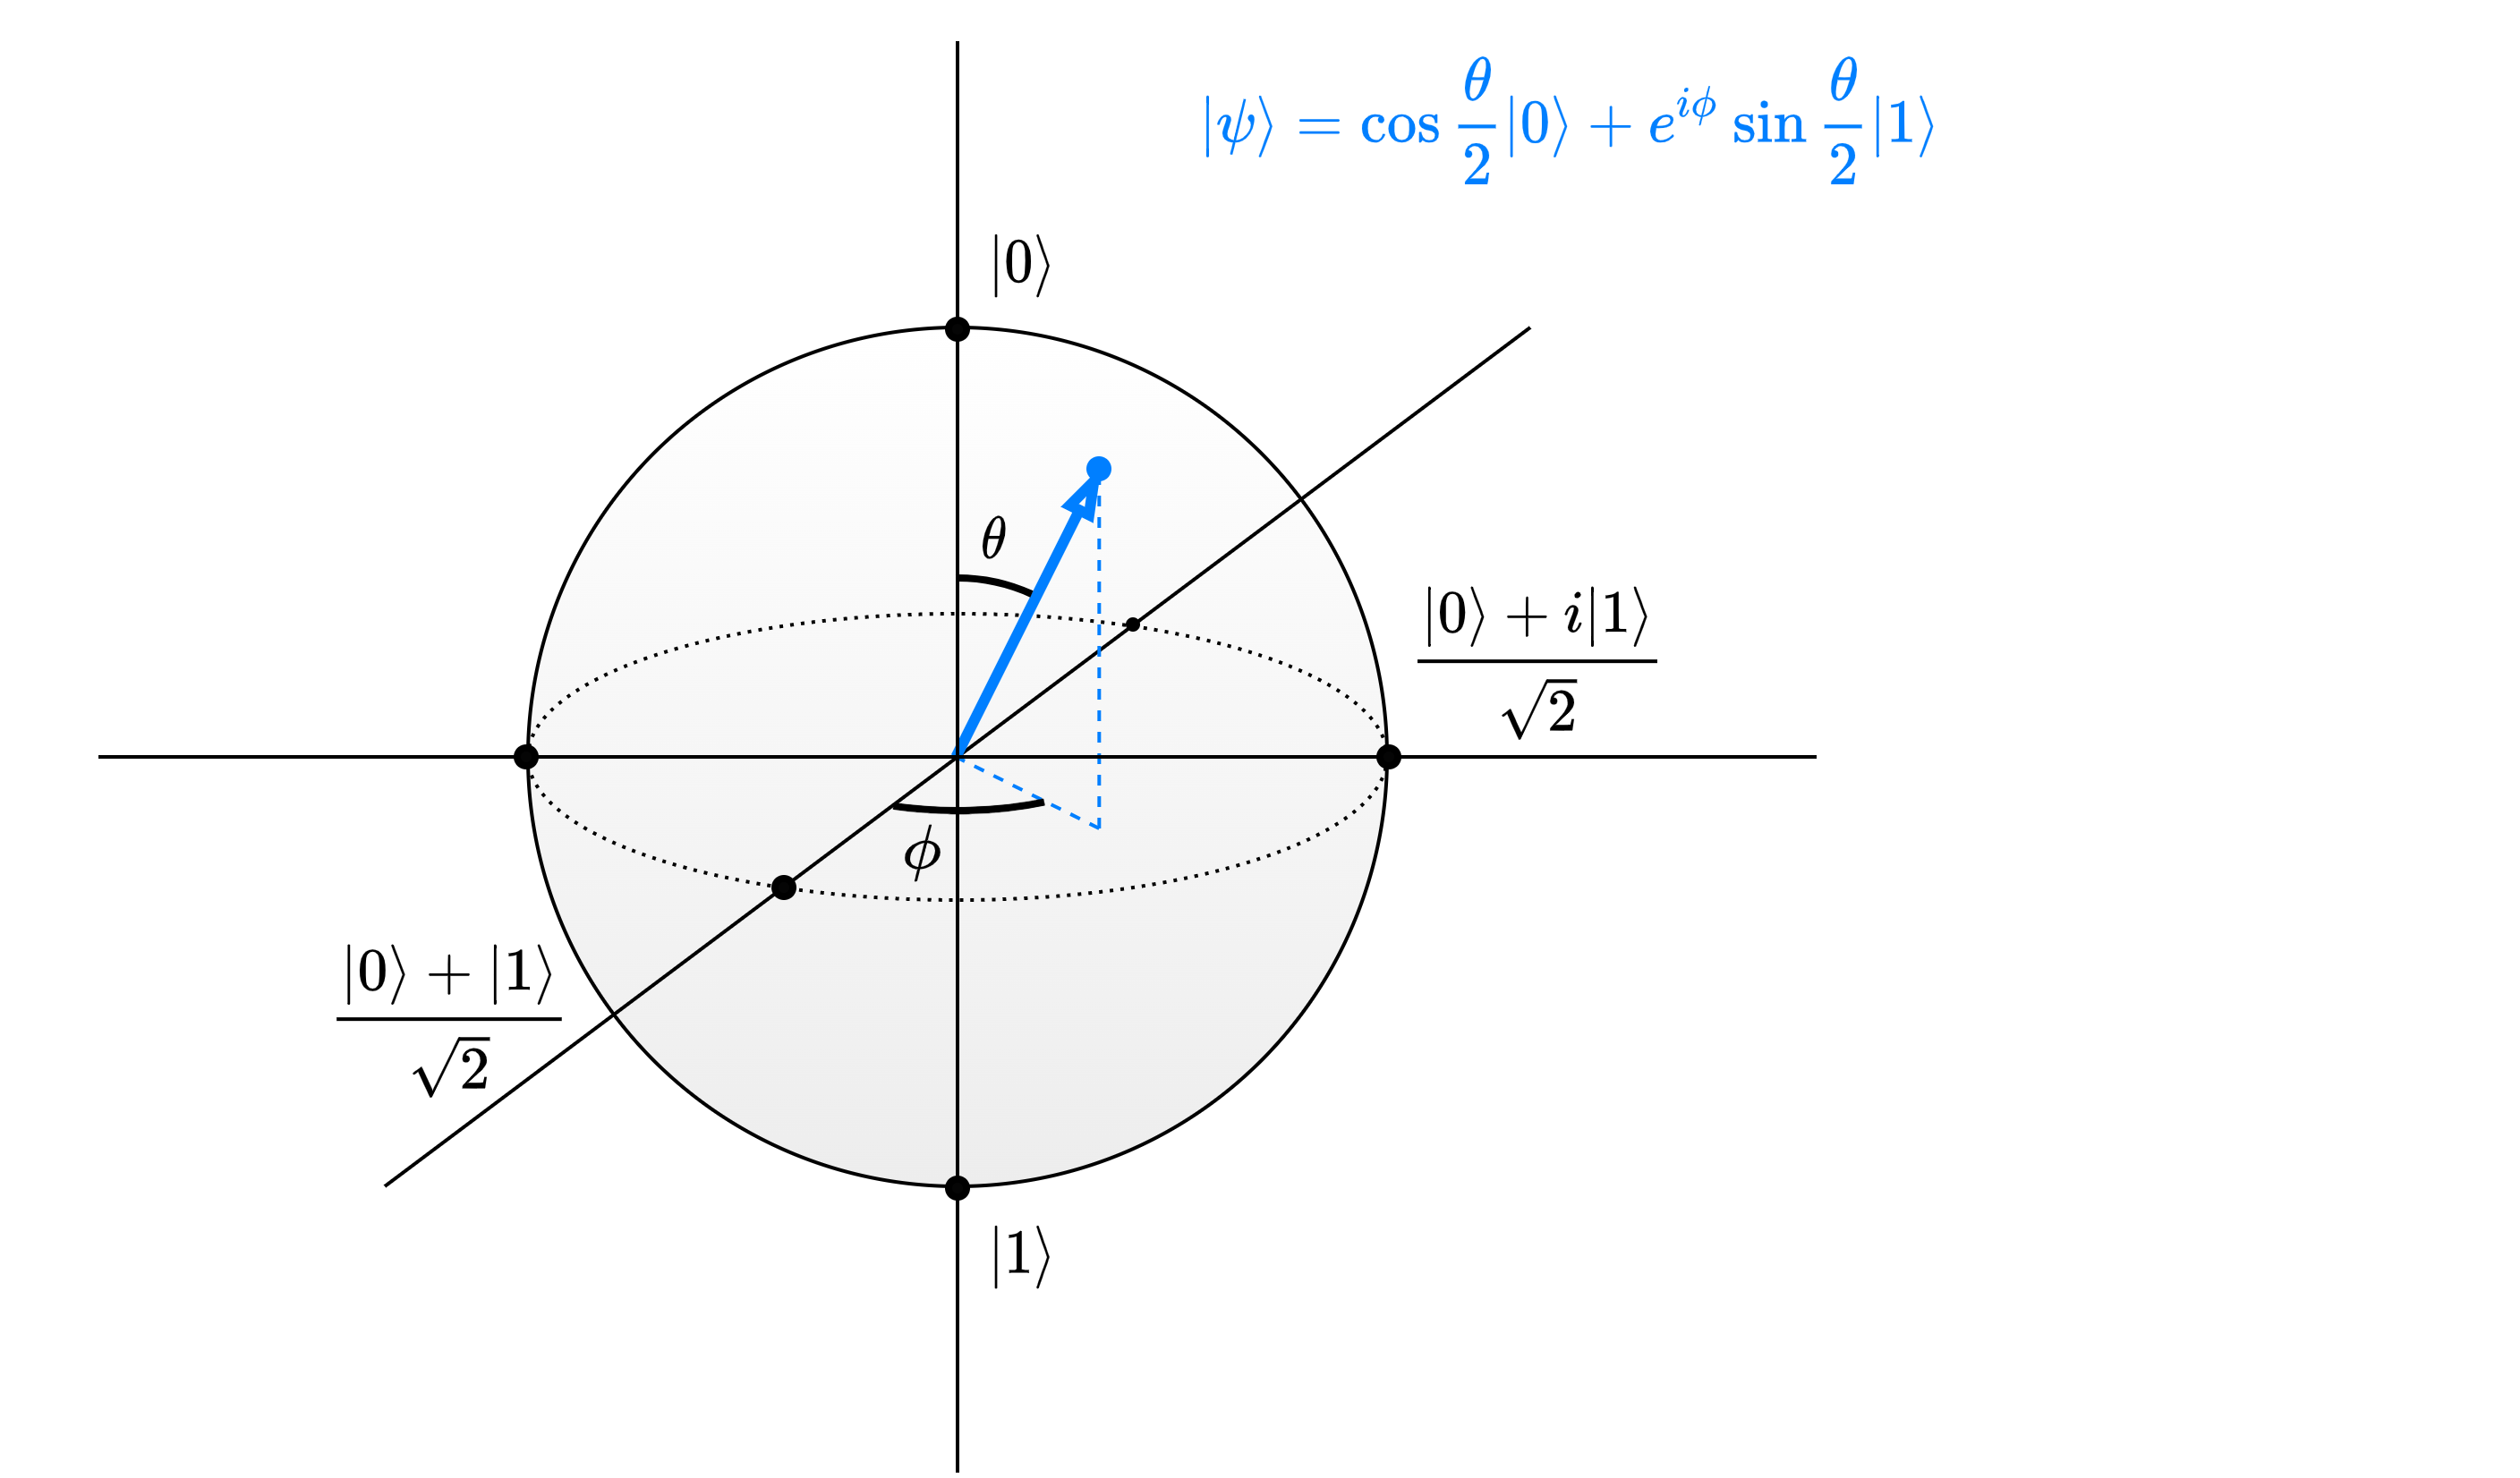
\includegraphics[scale=0.5]{bloch_sphere.png}
	\caption{The state of a single qubit can be visualized as a point on the Bloch sphere.}
\end{wrapfigure}
A qubit (quantum bit) is a \textbf{two-level quantum system}. In other words, there are only two possible states that we can measure the qubit to be in --- call them $\ket{0}$ and $\ket{1}$. When we perform a measurement of the qubit, we will always measure either $0$ or $1$. As the postulates say, these measurement outcomes must correspond to a Hermitian operator which we will call $\sigma_z$. The states $\ket{0}$ and $\ket{1}$ are the eigenstates of $\sigma_z$, which by the properties of Hermitian operators, form an orthonormal basis for the Hilbert space. Any arbitrary state in the Hilbert space $\mathscr{H}=\mathbb{C}^2$ can therefore be written
$$ \ket{\psi}=\alpha\ket{0} + \beta\ket{1} $$
for some complex coefficients $\alpha,\beta$ which are normalized so that $|\alpha|^2+|\beta|^2=1$. We say that the qubit is in a \textbf{superposition} of the $\ket{0}$ state and the $\ket{1}$ state. The postulates tell us that the probability of measuring a $0$ in this case is $p(0)=|\bra{0}\ket{\psi}|^2$. Plugging in the above form for $\ket{\psi}$ and using the orthogonality of the eigenvectors, we find $p(0) = |\alpha|^2$. Similarly $p(1)=|\beta|^2$. For this reason, the coefficients $\alpha$ and $\beta$ are called \textbf{probability amplitudes}. Note that they are \textbf{not} probabilities themselves --- they are complex after all --- but their squared modulus is a probability.\sidenote{Complex probability amplitudes are exactly what differentiates QM from ordinary probability. Indeed, complex values have phase and thereby allow interference phenomena which are fundamental to QM.}


\newpage


\section{Appendix}
\addcontentsline{toc}{section}{Appendix}
\subsection*{A1. Review of Complex Algebra}
A complex number is generally of the form $z=x+iy$ for real values $x,y\in\mathbb{R}$. The ``imaginary unit" $i$ is defined as the solution to $x^2+1=0$. Formally, we may write $i=\sqrt{-1}$. Complex numbers add as 
$$ z_1 + z_2 = x_1+x_2 + i(y_1+y_2) $$
and multiply as 
$$ z_1z_2 = (x_1+iy_1)(x_2+iy_2)= x_1x_2 - y_1y_2 + i(x_1y_2 + x_2y_1) $$
Complex conjugation, denoted by a star $^*$, is the replacement of $i$ by $-i$ everywhere it appears. So for $z=x+iy$, the conjugate is
$$ z^* = x - iy $$
The \textbf{modulus} of a complex number is defined by
$$ |z| = \sqrt{z^*z} = \sqrt{x^2+y^2} $$
Division by complex numbers is defined by
$$ \frac{z_1}{z_2} = \frac{z_2^*z_1}{z_2^*z_2} = \frac{z_2^*z_1}{|z_2|^2} $$





	
\end{document}